% Options for packages loaded elsewhere
\PassOptionsToPackage{unicode}{hyperref}
\PassOptionsToPackage{hyphens}{url}
\PassOptionsToPackage{dvipsnames,svgnames,x11names}{xcolor}
\documentclass[
  english,
  11pt,
]{article}
\usepackage{xcolor}
\usepackage[margin=1in]{geometry}
\usepackage{amsmath,amssymb}
\setcounter{secnumdepth}{-\maxdimen} % remove section numbering
\usepackage{iftex}
\ifPDFTeX
  \usepackage[T1]{fontenc}
  \usepackage[utf8]{inputenc}
  \usepackage{textcomp} % provide euro and other symbols
\else % if luatex or xetex
  \usepackage{unicode-math} % this also loads fontspec
  \defaultfontfeatures{Scale=MatchLowercase}
  \defaultfontfeatures[\rmfamily]{Ligatures=TeX,Scale=1}
\fi
\usepackage{lmodern}
\ifPDFTeX\else
  % xetex/luatex font selection
\fi
% Use upquote if available, for straight quotes in verbatim environments
\IfFileExists{upquote.sty}{\usepackage{upquote}}{}
\IfFileExists{microtype.sty}{% use microtype if available
  \usepackage[]{microtype}
  \UseMicrotypeSet[protrusion]{basicmath} % disable protrusion for tt fonts
}{}
\usepackage{setspace}
\makeatletter
\@ifundefined{KOMAClassName}{% if non-KOMA class
  \IfFileExists{parskip.sty}{%
    \usepackage{parskip}
  }{% else
    \setlength{\parindent}{0pt}
    \setlength{\parskip}{6pt plus 2pt minus 1pt}}
}{% if KOMA class
  \KOMAoptions{parskip=half}}
\makeatother
\usepackage{color}
\usepackage{fancyvrb}
\newcommand{\VerbBar}{|}
\newcommand{\VERB}{\Verb[commandchars=\\\{\}]}
\DefineVerbatimEnvironment{Highlighting}{Verbatim}{commandchars=\\\{\}}
% Add ',fontsize=\small' for more characters per line
\newenvironment{Shaded}{}{}
\newcommand{\AlertTok}[1]{\textcolor[rgb]{1.00,0.00,0.00}{\textbf{#1}}}
\newcommand{\AnnotationTok}[1]{\textcolor[rgb]{0.38,0.63,0.69}{\textbf{\textit{#1}}}}
\newcommand{\AttributeTok}[1]{\textcolor[rgb]{0.49,0.56,0.16}{#1}}
\newcommand{\BaseNTok}[1]{\textcolor[rgb]{0.25,0.63,0.44}{#1}}
\newcommand{\BuiltInTok}[1]{\textcolor[rgb]{0.00,0.50,0.00}{#1}}
\newcommand{\CharTok}[1]{\textcolor[rgb]{0.25,0.44,0.63}{#1}}
\newcommand{\CommentTok}[1]{\textcolor[rgb]{0.38,0.63,0.69}{\textit{#1}}}
\newcommand{\CommentVarTok}[1]{\textcolor[rgb]{0.38,0.63,0.69}{\textbf{\textit{#1}}}}
\newcommand{\ConstantTok}[1]{\textcolor[rgb]{0.53,0.00,0.00}{#1}}
\newcommand{\ControlFlowTok}[1]{\textcolor[rgb]{0.00,0.44,0.13}{\textbf{#1}}}
\newcommand{\DataTypeTok}[1]{\textcolor[rgb]{0.56,0.13,0.00}{#1}}
\newcommand{\DecValTok}[1]{\textcolor[rgb]{0.25,0.63,0.44}{#1}}
\newcommand{\DocumentationTok}[1]{\textcolor[rgb]{0.73,0.13,0.13}{\textit{#1}}}
\newcommand{\ErrorTok}[1]{\textcolor[rgb]{1.00,0.00,0.00}{\textbf{#1}}}
\newcommand{\ExtensionTok}[1]{#1}
\newcommand{\FloatTok}[1]{\textcolor[rgb]{0.25,0.63,0.44}{#1}}
\newcommand{\FunctionTok}[1]{\textcolor[rgb]{0.02,0.16,0.49}{#1}}
\newcommand{\ImportTok}[1]{\textcolor[rgb]{0.00,0.50,0.00}{\textbf{#1}}}
\newcommand{\InformationTok}[1]{\textcolor[rgb]{0.38,0.63,0.69}{\textbf{\textit{#1}}}}
\newcommand{\KeywordTok}[1]{\textcolor[rgb]{0.00,0.44,0.13}{\textbf{#1}}}
\newcommand{\NormalTok}[1]{#1}
\newcommand{\OperatorTok}[1]{\textcolor[rgb]{0.40,0.40,0.40}{#1}}
\newcommand{\OtherTok}[1]{\textcolor[rgb]{0.00,0.44,0.13}{#1}}
\newcommand{\PreprocessorTok}[1]{\textcolor[rgb]{0.74,0.48,0.00}{#1}}
\newcommand{\RegionMarkerTok}[1]{#1}
\newcommand{\SpecialCharTok}[1]{\textcolor[rgb]{0.25,0.44,0.63}{#1}}
\newcommand{\SpecialStringTok}[1]{\textcolor[rgb]{0.73,0.40,0.53}{#1}}
\newcommand{\StringTok}[1]{\textcolor[rgb]{0.25,0.44,0.63}{#1}}
\newcommand{\VariableTok}[1]{\textcolor[rgb]{0.10,0.09,0.49}{#1}}
\newcommand{\VerbatimStringTok}[1]{\textcolor[rgb]{0.25,0.44,0.63}{#1}}
\newcommand{\WarningTok}[1]{\textcolor[rgb]{0.38,0.63,0.69}{\textbf{\textit{#1}}}}
\usepackage{longtable,booktabs,array}
\usepackage{caption}
\captionsetup[table]{skip=6pt}
\newcounter{none} % for unnumbered tables
\usepackage{calc} % for calculating minipage widths
% Correct order of tables after \paragraph or \subparagraph
\usepackage{etoolbox}
\makeatletter
\patchcmd\longtable{\par}{\if@noskipsec\mbox{}\fi\par}{}{}
\makeatother
% Allow footnotes in longtable head/foot
\IfFileExists{footnotehyper.sty}{\usepackage{footnotehyper}}{\usepackage{footnote}}
\makesavenoteenv{longtable}
\usepackage{graphicx}
\makeatletter
\newsavebox\pandoc@box
\newcommand*\pandocbounded[1]{% scales image to fit in text height/width
  \sbox\pandoc@box{#1}%
  \Gscale@div\@tempa{\textheight}{\dimexpr\ht\pandoc@box+\dp\pandoc@box\relax}%
  \Gscale@div\@tempb{\linewidth}{\wd\pandoc@box}%
  \ifdim\@tempb\p@<\@tempa\p@\let\@tempa\@tempb\fi% select the smaller of both
  \ifdim\@tempa\p@<\p@\scalebox{\@tempa}{\usebox\pandoc@box}%
  \else\usebox{\pandoc@box}%
  \fi%
}
% Set default figure placement to htbp
\def\fps@figure{htbp}
\makeatother
% definitions for citeproc citations
\NewDocumentCommand\citeproctext{}{}
\NewDocumentCommand\citeproc{mm}{%
  \begingroup\def\citeproctext{#2}\cite{#1}\endgroup}
\makeatletter
 % allow citations to break across lines
 \let\@cite@ofmt\@firstofone
 % avoid brackets around text for \cite:
 \def\@biblabel#1{}
 \def\@cite#1#2{{#1\if@tempswa , #2\fi}}
\makeatother
\newlength{\cslhangindent}
\setlength{\cslhangindent}{1.5em}
\newlength{\csllabelwidth}
\setlength{\csllabelwidth}{3em}
\newenvironment{CSLReferences}[2] % #1 hanging-indent, #2 entry-spacing
 {\begin{list}{}{%
  \setlength{\itemindent}{0pt}
  \setlength{\leftmargin}{0pt}
  \setlength{\parsep}{0pt}
  % turn on hanging indent if param 1 is 1
  \ifodd #1
   \setlength{\leftmargin}{\cslhangindent}
   \setlength{\itemindent}{-1\cslhangindent}
  \fi
  % set entry spacing
  \setlength{\itemsep}{#2\baselineskip}}}
 {\end{list}}
\usepackage{calc}
\newcommand{\CSLBlock}[1]{\hfill\break\parbox[t]{\linewidth}{\strut\ignorespaces#1\strut}}
\newcommand{\CSLLeftMargin}[1]{\parbox[t]{\csllabelwidth}{\strut#1\strut}}
\newcommand{\CSLRightInline}[1]{\parbox[t]{\linewidth - \csllabelwidth}{\strut#1\strut}}
\newcommand{\CSLIndent}[1]{\hspace{\cslhangindent}#1}
\ifLuaTeX
\usepackage[bidi=basic,shorthands=off]{babel}
\else
\usepackage[bidi=default,shorthands=off]{babel}
\fi
\ifLuaTeX
  \usepackage{selnolig} % disable illegal ligatures
\fi
\setlength{\emergencystretch}{3em} % prevent overfull lines
\providecommand{\tightlist}{%
  \setlength{\itemsep}{0pt}\setlength{\parskip}{0pt}}
% Publication typography only; explicit figure numbers come from the manuscript.
\usepackage{caption}
\captionsetup{labelformat=empty}
\usepackage{etoolbox}
\BeforeBeginEnvironment{Shaded}{\begin{samepage}}
\AfterEndEnvironment{Shaded}{\end{samepage}}
\usepackage{bookmark}
\IfFileExists{xurl.sty}{\usepackage{xurl}}{} % add URL line breaks if available
\urlstyle{same}
% fallback for those not using the hyperref driver hyperxmp:
\makeatletter
\@ifundefined{xmpquote}{\newcommand{\xmpquote}[1]{#1}}{}
\makeatother
\hypersetup{
  pdftitle={Pelagic: A Real-Time Mathematical Rendering System for Procedural Jellyfish{,} Stateful Appendages{,} Underwater Optics{,} and Interactive Liquid Glass},
  pdfauthor={Mani Marami Milani},
  pdflang={en},
  colorlinks=true,
  linkcolor={teal},
  filecolor={Maroon},
  citecolor={Blue},
  urlcolor={teal},
  pdfcreator={LaTeX via pandoc}}

\title{Pelagic: A Real-Time Mathematical Rendering System for Procedural
Jellyfish, Stateful Appendages, Underwater Optics, and Interactive
Liquid Glass}
\author{Mani Marami Milani}
\date{Technical preprint · 2026 · Local publication-review edition}

\begin{document}
\maketitle

\setstretch{1.04}
\section{Abstract}\label{abstract}

Real-time organism scenes become difficult to maintain when anatomy,
motion, environmental effects, camera control and interface optics
evolve as unrelated demonstrations. Pelagic is a browser-based rendering
study that connects these systems while preserving an art-directed
jellyfish identity. Its implementation combines a procedural mantle and
folded oral membranes, pulse-coupled locomotion, persistent constrained
appendages, bounded world-space currents, projected-size population
detail, and an input-driven six-degree-of-freedom camera journey. A
shared optical compositor samples one live ocean image for refractive
bubbles, localized thermal shimmer and an interactive liquid clock. The
clock combines authored implicit-surface choreography with a
low-resolution persistent spring/advection field. This paper describes
the actual Three.js 0.175.0 implementation, distinguishes
code-equivalent equations from abstractions and artistic heuristics, and
links the methods to reproducible source locations. The accompanying
artifact includes browser motion evidence, deterministic tests,
historical rejected approaches and fresh frame-interval measurements of
the approved runtime. The work is a systems and visual-engineering
study, not a fluid--structure interaction model, calibrated biological
simulation or claim of algorithmic priority. Image-space optics cannot
recover unseen radiance; liquid topology is not mass-conserving;
performance and compatibility evidence remain specific to the tested
hardware and backend.

\section{1. Introduction}\label{introduction}

Pelagic presents a quiet underwater scene rather than a conventional
portfolio of interface panels. Jellyfish move through open water, an
input-driven camera visits several compositions, a brief bubble passage
bends the live image, and a deep basalt sanctuary supplies a different
scale of environmental detail. After inactivity, the same moving ocean
becomes the source image for a liquid clock. These changes create a
useful engineering problem: the visual identity must survive changes in
scale, orientation, detail level and optical treatment.

A compelling still is insufficient. A rim can look continuous at rest
yet break under contraction. A membrane may resemble tissue from the
front but reveal a flat strip underneath. A distant animal can have a
smooth silhouette while its appendages rotate rigidly with its body. A
transparent clock can look luminous without bending anything beneath it.
Pelagic's development therefore relied on controlled motion checks as
well as attractive views. Figure 1 introduces the runtime; the motion
supplement separates the behaviors that a still cannot prove.

The publication has a narrower claim than the ambition of the artwork.
It documents one implemented system and its tradeoffs. It does not
compare itself numerically with unrelated graphics demos, report
user-study outcomes, or infer physical fidelity from resemblance. The
authoritative runtime is commit
\texttt{bce3571b0300ecfe5dc6e5dd45f28a9cda57006e}. Publication commits
add explanation, measurement and packaging without changing that
artwork. An unapproved later background experiment is discussed only as
supplemental negative evidence.

\begin{figure}
\centering
\pandocbounded{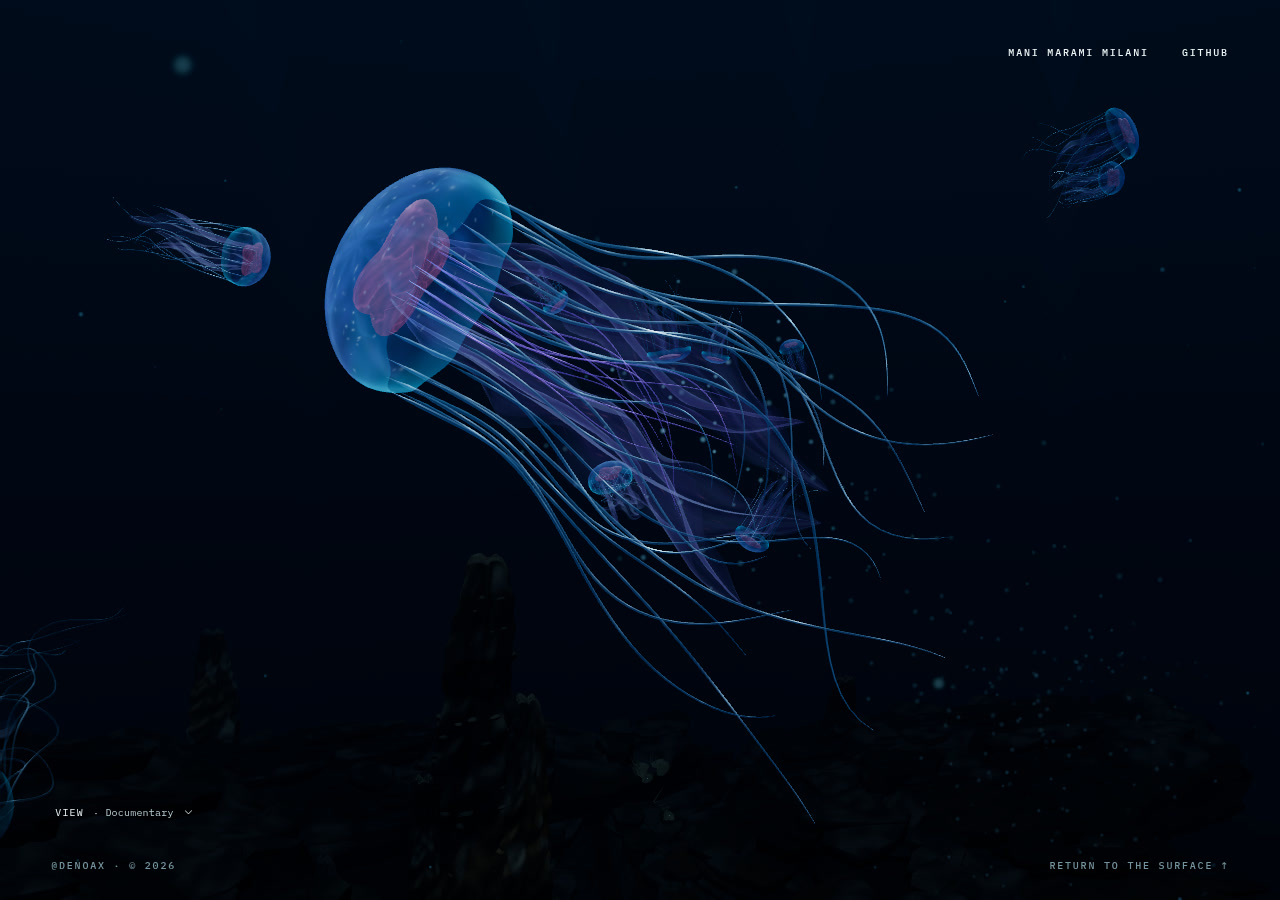
\includegraphics[keepaspectratio,alt={Figure 1. Approved-runtime overview: luminous procedural tissue within the shared ocean. Actual browser capture; camera state and renderer metadata accompany the figure.}]{figures/F01-overview.jpg}}
\caption{Figure 1. Approved-runtime overview: luminous procedural tissue
within the shared ocean. Actual browser capture; camera state and
renderer metadata accompany the figure.}
\end{figure}

\section{2. Contributions}\label{contributions}

The contribution is the documented integration and its inspectable
artifact, not a new physical law. Five aspects organize the paper:

\begin{enumerate}
\def\labelenumi{\arabic{enumi}.}
\tightlist
\item
  A shared anatomical surface contract for the bell, rolled margin and
  appendage roots, paired with folded membranes and stateful transport.
\item
  A pulse state reused for deformation and propulsion, observed by a
  bounded current/wake system rather than replaced by an independent
  decorative halo.
\item
  Population detail that follows projected importance while retaining
  the approved tissue implementation and persistent appendage state.
\item
  One live-ocean optical source shared by bubbles, thermal shimmer and
  idle glass, with explicit approximation boundaries and resource
  ownership.
\item
  A reproducible account of source-derived mathematics, motion checks,
  performance, rejected designs and remaining limitations.
\end{enumerate}

Each is an engineering result. The equations are deliberately modest:
familiar building blocks become useful when their coordinate spaces,
timing and ownership are made consistent. Table 1 identifies those
responsibilities.

\section{3. Related work and scope of
influence}\label{related-work-and-scope-of-influence}

The biological literature distinguishes mechanisms that a stylized
animation can easily collapse into a single sinusoid. Costello and
colleagues review jellyfish swimming across morphological and
hydrodynamic regimes (\citeproc{ref-costello2021}{Costello et al.
2021}). Gemmell and colleagues describe passive energy recapture during
refill (\citeproc{ref-gemmell2013}{Gemmell et al. 2013}). These sources
motivate a distinction between contraction, recovery and coast. Pelagic
does not reproduce their experimental apparatus, pressure fields,
efficiency measurements or species-specific kinematics. Its secondary
thrust is an authored temporal signal, not an estimate of recovered
energy.

Position-based dynamics provides relevant context for correcting
geometric constraints after a prediction step
(\citeproc{ref-muller2007}{Müller et al. 2007}). Pelagic's appendages
use previous positions, damping and repeated length projection. They do
not implement the complete general method, derive compliance from tissue
measurements, or solve a coupled elastic volume. A small oral-spine
separation operation is a visual contact heuristic, not a comprehensive
self-collision system.

Blinn's implicit surfaces establish the usefulness of summing smooth
density functions to form connected shapes
(\citeproc{ref-blinn1982}{Blinn 1982}). Pelagic applies additive
implicit contributions to a two-dimensional clock field. No
three-dimensional isosurface is extracted, and the apparent liquid
volume is not conserved. Image-space refraction work, including Wyman's
two-interface approximation (\citeproc{ref-wyman2005}{Wyman 2005}),
supplies a useful conceptual boundary: plausible optical images can be
produced without complete scene transport, but missing image information
remains missing. Pelagic solves analytic ellipsoid interfaces and
samples its current ocean image; it is not a reproduction of Wyman's
entire pipeline.

The software foundation includes an adapted MIT-licensed Aurelia scene
(\citeproc{ref-aurelia}{Niehus, n.d.}) and the pinned Three.js renderer
(\citeproc{ref-three175}{Three.js contributors 2025}). FluidGlass was
studied as an interaction reference
(\citeproc{ref-fluidglass}{{chiuhans111}, n.d.}), not copied as source,
shader, layout or media. These implementation and design references are
not scientific validation. Third-party provenance and retained notices
accompany the artifact.

\section{4. System overview}\label{system-overview}

React owns readiness, idle intent and sparse semantic controls.
High-frequency work belongs to imperative scene objects and persistent
buffers. The scene uses \texttt{WebGPURenderer} from
\texttt{three/webgpu}, with an explicitly verified WebGL2 backend for
this publication. A package dependency on React Three Fiber does not
make this an R3F renderer: no Fiber scene ownership is used on the
active path.

The frame reads input and updates bounded journey progress. The school
director advances animal poses; the environment advances its persistent
populations; the detail adapter evaluates screen importance.
Connected-ocean state observes the animals and updates particulate.
Tissue geometry and presentation then update, followed by the existing
scene render. When optical effects are active, that render targets a
clean color image and a shared output pass composes the effects. Idle
adds small field-simulation passes, not another ocean.

\textbf{Table 1. Active responsibilities at the publication runtime.}

{\def\LTcaptype{none} % do not increment counter
\begin{longtable}[]{@{}
  >{\raggedright\arraybackslash}p{(\linewidth - 4\tabcolsep) * \real{0.3333}}
  >{\raggedright\arraybackslash}p{(\linewidth - 4\tabcolsep) * \real{0.3333}}
  >{\raggedright\arraybackslash}p{(\linewidth - 4\tabcolsep) * \real{0.3333}}@{}}
\toprule\noalign{}
\begin{minipage}[b]{\linewidth}\raggedright
Responsibility
\end{minipage} & \begin{minipage}[b]{\linewidth}\raggedright
Owner
\end{minipage} & \begin{minipage}[b]{\linewidth}\raggedright
Persistent state
\end{minipage} \\
\midrule\noalign{}
\endhead
\bottomrule\noalign{}
\endlastfoot
Browser/scene lifecycle & \texttt{HeroScene}, \texttt{useIdleScreen} &
renderer, scene, idle intent, readiness \\
Main route poses & \texttt{JellySchoolDirector} & position, velocity,
heading, pulse \\
Tissue & \texttt{LivingAppendages}, \texttt{PopulationAnimal} & chains,
geometry, material uniforms \\
Detail assignment & \texttt{PopulationDetail} & detail state, pooled
light/fleck ownership \\
Connected water & \texttt{CurrentField}, \texttt{ConnectedOcean},
\texttt{OceanSnow} & event pools and particle positions \\
Camera & \texttt{JourneyController}, \texttt{TrackPlayer},
\texttt{ViewController} & scalar progress, baked poses, Explore state \\
Optical output & \texttt{LiveOceanLens} & clean scene target and output
material \\
Sanctuary & \texttt{Sanctuary}, \texttt{VentDynamics} & geology
resources, plume, pooled illumination \\
Idle & \texttt{OceanIdleGlass}, \texttt{IdleDisplacement} & two masks,
two field targets, bounded choreography \\
\end{longtable}
}

\begin{figure}
\centering
\pandocbounded{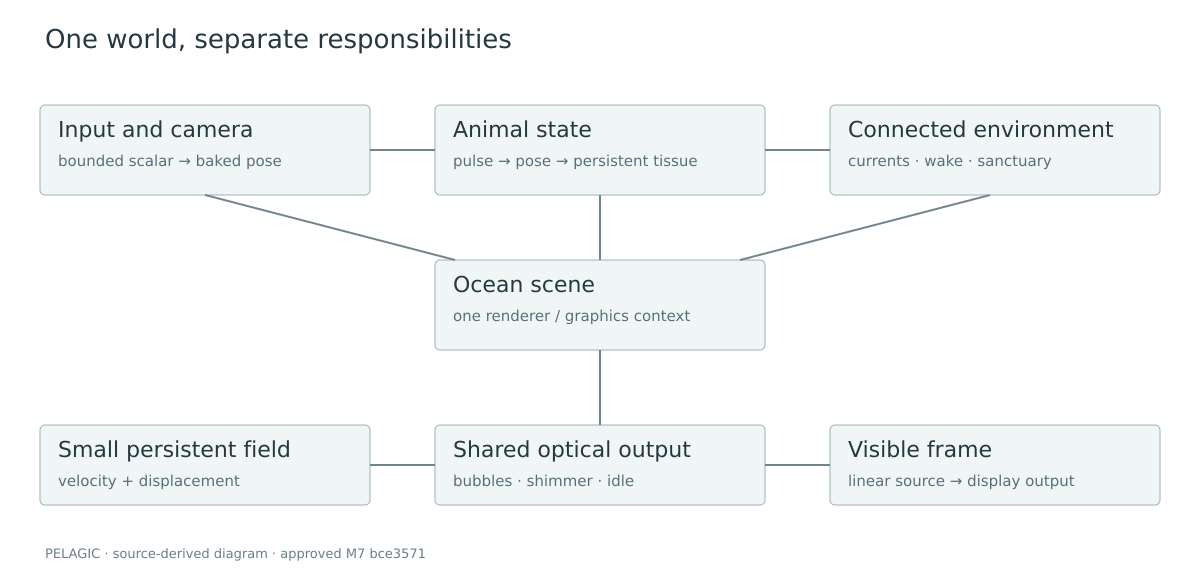
\includegraphics[keepaspectratio,alt={Figure 2. Ownership and frame composition. Auxiliary field/output draws are not additional ocean scene renders.}]{figures/F02-system.png}}
\caption{Figure 2. Ownership and frame composition. Auxiliary
field/output draws are not additional ocean scene renders.}
\end{figure}

\section{5. Notation and spaces}\label{notation-and-spaces}

World coordinates are right-handed with Y up. The bell-first animal axis
is local +Y, with X/Z spanning the rim. Appendage positions are
animal-local, but their previous state is transported to preserve
world-relative lag. Camera view direction is −Z. Output UV is
top-origin; the projection code explicitly inverts clip Y. Canvas
clock-mask sampling performs its own Y inversion.

Time is in seconds, except normalized pulse phase \(q\) and journey
progress \(s\). World lengths are artistic units, not meters. \(h\)
denotes a fixed simulation step. The mantle uses latitude parameter
\(\tau\) and azimuth \(\theta\); \(u\) is a transverse membrane
coordinate. \(S(x)\) denotes cubic smoothstep after clamping \(x\) to
\([0,1]\). The complete symbol table is in \texttt{notation.md}.

An equation labeled \textbf{CODE-EQUIVALENT} matches the stated source
subexpression, including its constants. It need not describe every
surrounding branch. A \textbf{CONTINUOUS ABSTRACTION} summarizes an
algorithm without claiming bitwise equivalence. An \textbf{ART-DIRECTION
HEURISTIC} expresses a designed relationship, not a physical inference.
These labels describe different questions from correctness: an exact
transcription can still be physically approximate.
\texttt{source-map.md} records immutable paths and line ranges for every
equation.

\section{6. Procedural jellyfish
geometry}\label{procedural-jellyfish-geometry}

\subsection{6.1 Mantle and root
continuity}\label{mantle-and-root-continuity}

The bell and rim share \texttt{mantlePoint}. Let \(R,H\) be
pulse-adjusted radius and height, \(p\) the bell contraction, \(L\) the
lobe count, \(y_r\) the rim offset and \(m_r\) the margin-roll signal.
Let \(c_x,c_y\) be the two-component local surface current. With
\(m=\tau^5\) and \(f=\cos(L\theta)\), equation (1) is
\textbf{CODE-EQUIVALENT}:

\[
\begin{aligned}
\rho&=\sin(\pi\tau/2)R(1-0.07pm)(1+0.012fm),\\
x&=\cos\theta\,\rho+0.08c_x\tau^2,\\
y&=\cos(\pi\tau/2)H+y_r\tau^2+m(0.014f+0.04m_r),\\
z&=\sin\theta\,\rho+0.08c_y\tau^2.
\end{aligned}
\]

\(\tau=0\) is the apex; \(\tau=1\) is the equatorial region; the surface
extends to a softly rolled margin near \(1.12\). Rim tentacles attach at
\(1.1\) on this same function. This avoids tuning disconnected rim
geometry against the bell. Periodicity in \(\theta\) is maintained while
the bell contracts. Seam normals and fractional-power domains require
separate numerical care: a valid surface does not prevent a shader NaN
from appearing as a black seam.

\subsection{6.2 Folded oral membranes}\label{folded-oral-membranes}

An oral arm is not merely a wide line. Its simulated spine carries a
transverse folded section with narrowed insertion and rounded tip. For
normalized length \(t\in[0,1]\), transverse \(u\in[-1,1]\), arm index
\(a\), and animation phase \(\phi\), equation (2) is
\textbf{CODE-EQUIVALENT}:

\[
\begin{aligned}
w&=(0.055+0.32\sin(\pi t)^{0.65})\sqrt{\max(0,1-t^8)},\\
b&=uw[1+0.20|u|\sin(30t-a)],\\
f&=[\sin(2\pi u+7t+a)-\sin(7t+a)]\,0.30w\\
 &\quad+0.32w|u|^2\sin(30t+2u-a)
 +0.04w|u|\sin(22t-0.8a-0.42\phi).
\end{aligned}
\]

The section is reconstructed in a frame along the spine. The subtraction
in the first fold term keeps the central spine on its simulated
centerline. Free-edge terms add folding without moving the whole arm as
an independent object. The procedure remains a surface approximation:
intersections can occur because folded sheets have no volumetric
collision solver.

\begin{figure}
\centering
\pandocbounded{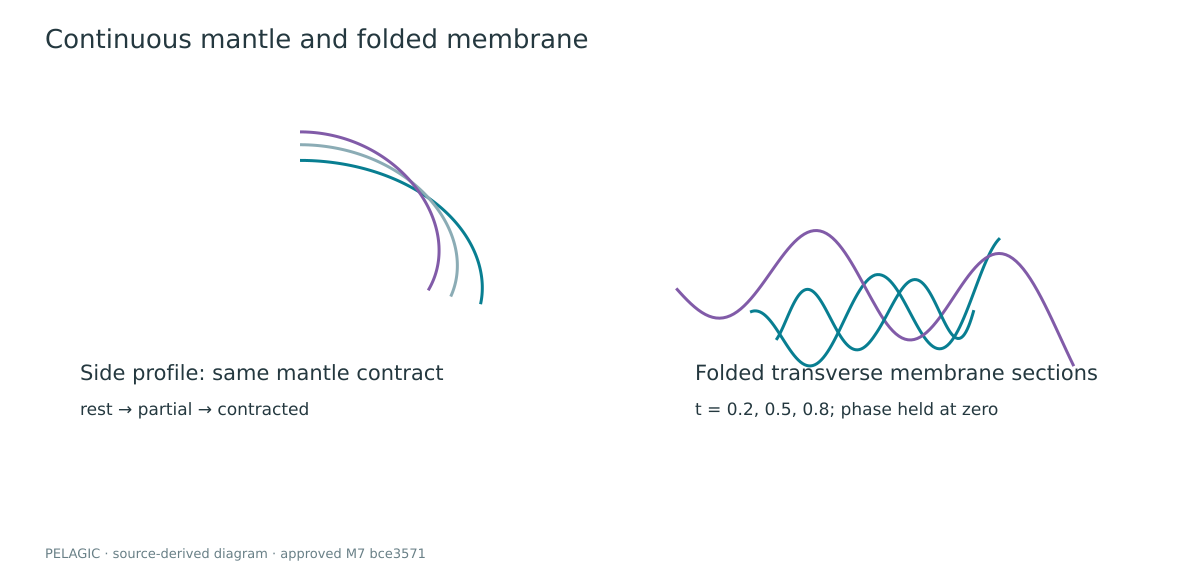
\includegraphics[keepaspectratio,alt={Figure 3. Mantle coordinates and folded section, plotted from the approved functions rather than traced from a screenshot.}]{figures/F03-anatomy.png}}
\caption{Figure 3. Mantle coordinates and folded section, plotted from
the approved functions rather than traced from a screenshot.}
\end{figure}

\section{7. Bell kinematics}\label{bell-kinematics}

The normalized swim phase wraps continuously. Contraction occupies the
first 0.20 of the cycle, refill continues to 0.68, and the remaining
interval is a coast. Equation (3), \textbf{CODE-EQUIVALENT}, defines
contraction magnitude:

\[
p(q)=\begin{cases}
S(q/0.20),&q<0.20,\\
1-[S((q-0.20)/0.48)]^{1.42},&0.20\le q<0.68,\\
0,&q\ge0.68.
\end{cases}
\]

Define a window \(W(q;a,b)=\sin^2[\pi(q-a)/(b-a)]\) strictly inside
\((a,b)\) and zero elsewhere. Equation (4), \textbf{CODE-EQUIVALENT},
gives primary thrust \(T_1=W(q;0.025,0.215)\), secondary thrust
\(T_2=W(q;0.57,0.82)\), and margin roll
\(m_r=0.78T_1-0.52W(q;0.22,0.66)\).

The same state reaches geometry and locomotion. It produces a temporal
relationship, not a claim of measured pressure. Activation adds an
integrated response through the existing tissue state rather than
creating a replacement animal. Figure 4 plots the exact signals; S1
supplies the corresponding motion; S1 shows several cycles without
converting timing into a still-image claim.

\begin{figure}
\centering
\pandocbounded{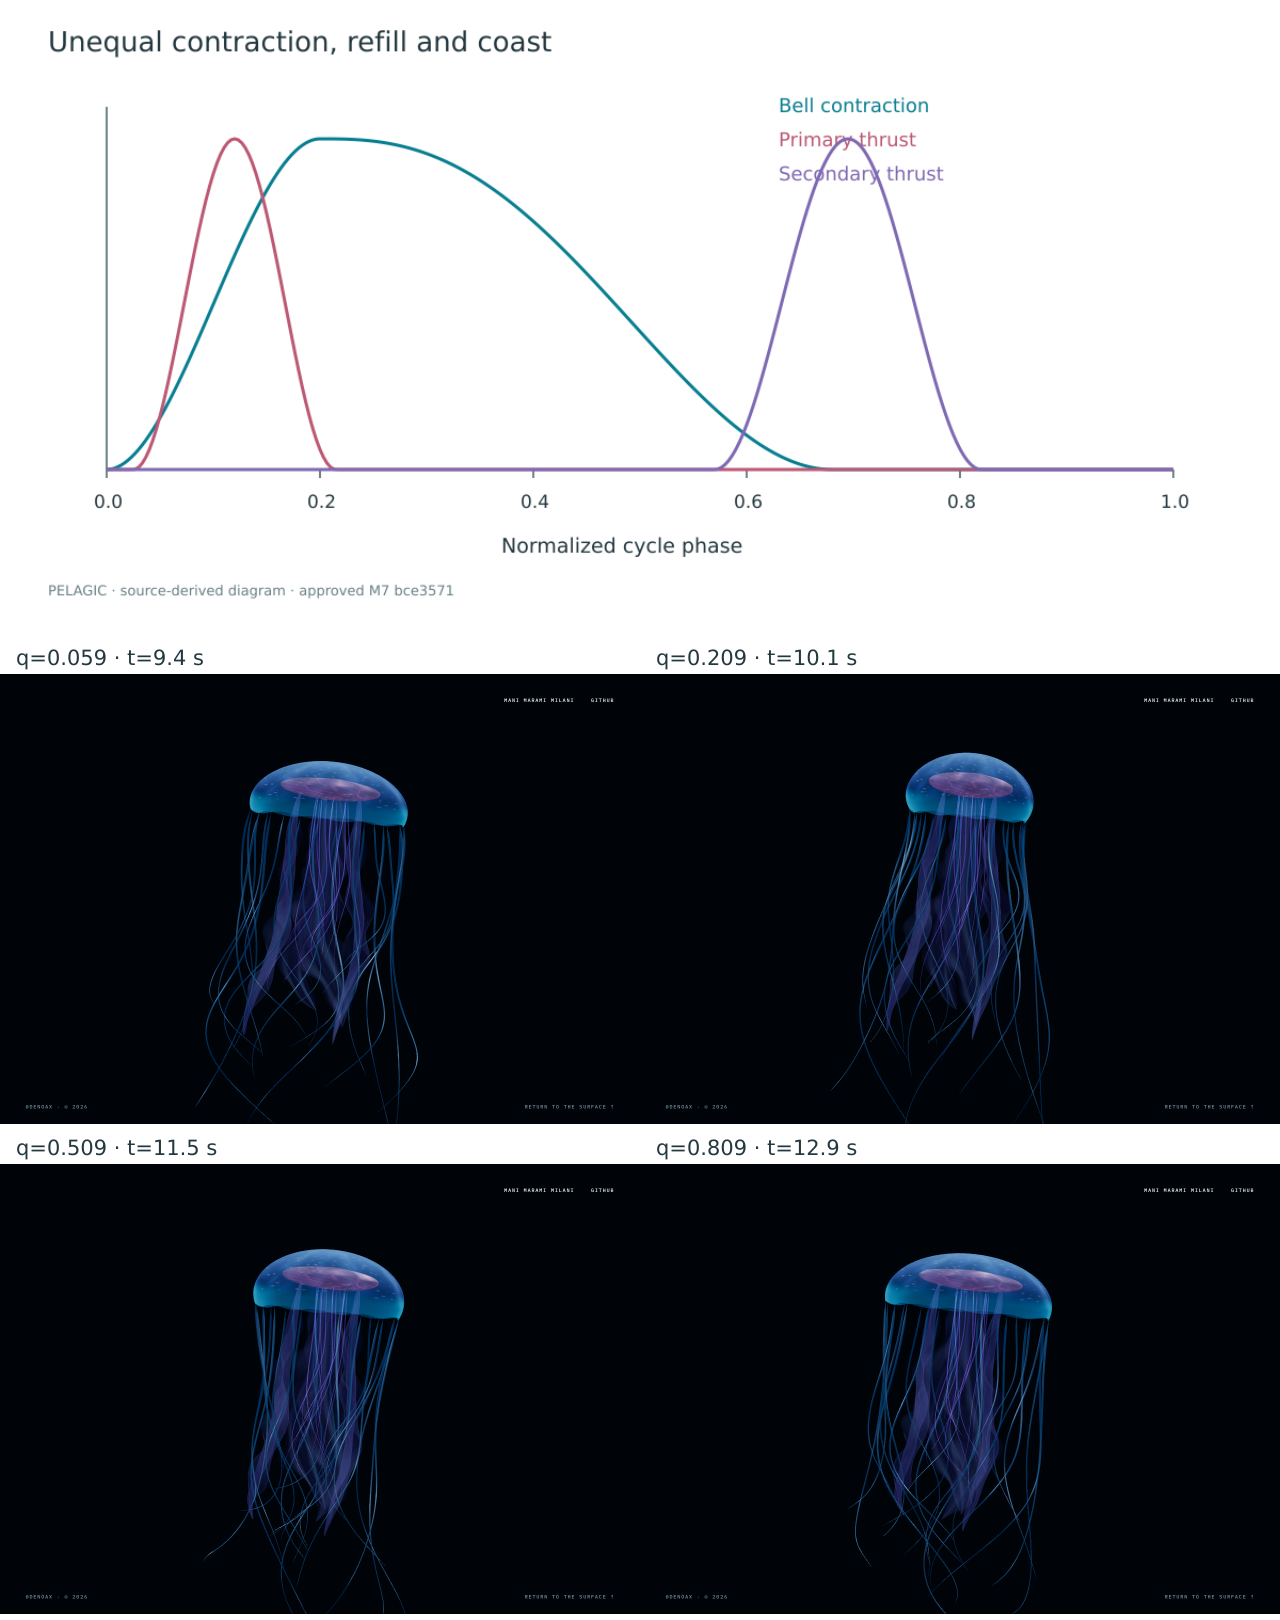
\includegraphics[keepaspectratio,alt={Figure 4. Exact source-derived pulse curves and four actual browser poses with recorded phase q and simulation time. Fixed specimen view and distance; contraction, refill and coast are unequal. S1 supplies continuous motion.}]{figures/F04-pulse.png}}
\caption{Figure 4. Exact source-derived pulse curves and four actual
browser poses with recorded phase q and simulation time. Fixed specimen
view and distance; contraction, refill and coast are unequal. S1
supplies continuous motion.}
\end{figure}

\section{8. Locomotion and schooling}\label{locomotion-and-schooling}

Each main-route animal has a desired location derived from an authored
path plus slow current-like variation. Its position is integrated from
velocity; it is not simply placed on that desired point each frame. The
direction blends toward the route with a contraction-dependent gain. In
equation (5), \textbf{CODE-EQUIVALENT} for the velocity core, \(\hat d\)
is the updated swimming direction, \(e=X_{desired}-X\),
\(k=\min(0.42,0.075+0.045\|e\|)\),
\(a=(0.72+0.28\,scale)\,motionScale\), and \(c\) is the two-dimensional
current:

\[
\begin{aligned}
V^*&=V+h[(2.35T_1+0.58T_2)a\hat d+ke
          +0.095\,motionScale(c_x,0,c_y)],\\
V^+&=\operatorname{cap}_{v_{max}}\{V^*e^{-h(0.24+0.22\,refill-0.08\,coast)}\},\\
X^+&=X+hV^+.
\end{aligned}
\]

The cap is \(v_{max}=0.92+0.42\,drift\). A separate soft composition
correction engages when route error exceeds 4.2 world units; excluding
it would overstate the purity of propulsion-driven travel. Orientation
follows velocity with a pulse-dependent quaternion blend. No calibrated
body drag or added-mass model is implied by the exponential factor.

For pairs of visible main-route animals, equation (6),
\textbf{CODE-EQUIVALENT}, adds opposite desired-position corrections
when \(d<d_{safe}\):

\[
C_{ij}=0.44(1-d/d_{safe})\frac{X_{desired,i}-X_{desired,j}}{d},
\qquad d_{safe}=1.05+0.55(scale_i+scale_j).
\]

Distance is clamped below at 0.001. This steers desired routes apart; it
does not resolve collisions between all membranes or represent a general
schooling model. The distant route source has its own established motion
history; the population adapter shares rendering quality, not a newly
unified route solver.

\textbf{Algorithm 1 --- animal update (structural pseudocode).}

\begin{Shaded}
\begin{Highlighting}[]
\NormalTok{evaluate authored desired route and bounded drift}
\NormalTok{accumulate pairwise desired{-}route separation}
\NormalTok{sample contraction/refill/coast state}
\NormalTok{turn swimming direction toward desired route}
\NormalTok{integrate pulse thrust, weak tether and current into velocity}
\NormalTok{apply drag and speed cap; integrate position}
\NormalTok{apply exceptional soft composition guard if far outside route}
\NormalTok{orient bell{-}first axis toward velocity; preserve physical scale}
\NormalTok{publish pose and pulse for tissue and environmental observers}
\end{Highlighting}
\end{Shaded}

\section{9. Stateful appendages}\label{stateful-appendages}

The appendage history is meaningful only if it survives body movement.
Before local simulation, current and previous points are rotated by the
change from the previous body frame and translated by the same inverse
body displacement. Applying a different transport to previous state
would inject spurious velocity. Large discontinuous body displacements
are guarded instead of replayed as a violent chain impulse.

Equation (7) is \textbf{CODE-EQUIVALENT} for prediction. With \(\sigma\)
the bounded frame scale and \(d_0=0.955\) for arms or \(0.968\) for
tentacles,

\[
\widetilde x_i=x_i+d_0^{\sigma}(x_i-x_i^-)+g_i+c_i+e_i+r_i.
\]

The named increments are not a single physically measured acceleration:
\(g_i\) is downward bias proportional to \(\sigma^2\); \(c_i\) is
current displacement proportional to longitudinal \(t_i^2\sigma^2\);
\(e_i\) is bounded traveling flow; \(r_i\) is a localized pointer
repulsion. The approved path uses \(h=1/60\), giving \(\sigma=1\) during
fixed simulation steps. Replacing these mixed increments by an
unexplained \(h^2F\) would misstate the implementation.

Roots are reattached during projection. For segment vector
\(\delta=x_i-x_{i-1}\), \(\ell=\max(10^{-4},\|\delta\|)\) and rest
length \(r\), equation (8), \textbf{CODE-EQUIVALENT}, is

\[
\epsilon=(\ell-r)/\ell,\qquad
x_{i-1}\leftarrow x_{i-1}+0.46\epsilon\delta,\quad
x_i\leftarrow x_i-0.54\epsilon\delta.
\]

The first free point instead receives the full correction because its
parent is fixed. Arms use five iterations, tentacles four. Three
oral-spine separation passes inspect neighboring longitudinal samples
and apply the same bounded correction to both Verlet histories. This
reduces some oblique crossings without adding artificial propulsion; it
is not sheet-sheet collision.

Visible tubes use frames transported along the chains. Folded arm
surfaces use the simulated centerline, not independent animation
transforms. Normal refresh and deformation scheduling depend on
significance; detail transitions resample the same state. S2 shows
turning and lag. Figure 5 distinguishes state from reconstructed surface
so a smooth mesh is not mistaken for a denser solver.

\begin{figure}
\centering
\pandocbounded{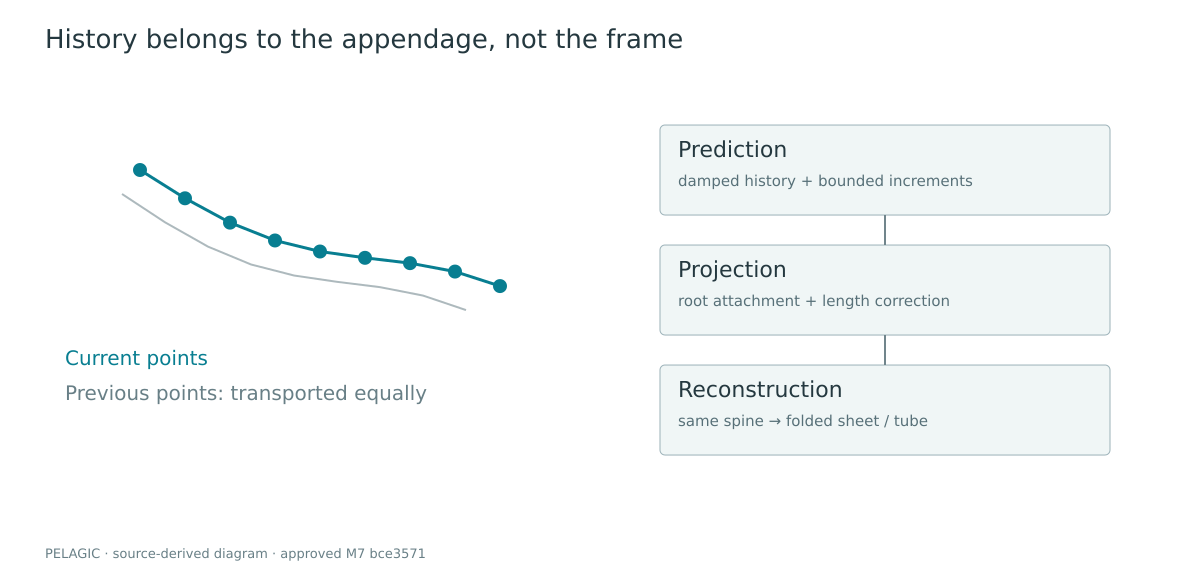
\includegraphics[keepaspectratio,alt={Figure 5. Persistent chain history, length projection and reconstructed membrane/tube surfaces.}]{figures/F05-appendages.png}}
\caption{Figure 5. Persistent chain history, length projection and
reconstructed membrane/tube surfaces.}
\end{figure}

\textbf{Algorithm 2 --- appendage step.}

\begin{Shaded}
\begin{Highlighting}[]
\NormalTok{transport both position histories into the current animal frame}
\NormalTok{accumulate bounded time; take fixed tissue steps}
\NormalTok{for each active chain:}
\NormalTok{    attach root to approved anatomy}
\NormalTok{    predict free points from damped history and authored increments}
\NormalTok{    repeat length projection; reattach root}
\NormalTok{separate nearby oral spines, correcting both histories equally}
\NormalTok{resample existing chains at the visible detail level}
\NormalTok{reconstruct folded membranes and tapered tubes; refresh needed normals}
\end{Highlighting}
\end{Shaded}

\section{10. Tissue optics and
bioluminescence}\label{tissue-optics-and-bioluminescence}

The bell uses \texttt{MeshPhysicalNodeMaterial}, but its translucent
identity is an explicit approximation. The material sets transmission to
zero: it does not refract the ocean framebuffer. Anatomical thickness,
facing and absorption control alpha, pigmentation and roughness. This
distinction matters because a living-looking bell is not evidence of
physical subsurface transport.

For clamped UV latitude \(v\), let \(K\) be the canal mask and
\(f=\max(0.24,|n_v\cdot v_{eye}|)\). Equation (9),
\textbf{CODE-EQUIVALENT} for the bell path, is

\[
\begin{aligned}
d_t&=0.30(1-v)^{1.4}+0.04+0.20K\max(0,\sin\pi v),\\
A&=1-e^{-1.7d_t/f},\\
\alpha&=\operatorname{clamp}_{[0.025,0.62]}
 [(0.40A+0.08)\,opacity/0.58].
\end{aligned}
\]

The membrane branch uses a different thickness/edge profile. UV clamps
protect fractional powers against tiny interpolation overshoots. This is
an important example of a defect that could resemble geometry
segmentation while originating in material evaluation.

A seeded 512×256 data texture stores soft mottling, canal structure and
sparse luminous cells in separate channels. It includes 112 seeded cell
marks and matching seam texels, with mipmapping for distance. Emission
has a hierarchy: soft tissue, brighter rim, pink/violet internal accents
and restrained speckles. A broad analytic environment lobe provides a
moving highlight as normals turn. Bloom is not used to construct the
animal; the inherited bloom chain is off.

The colors are art direction, not species spectroscopy. Double-sided
alpha surfaces can still sort imperfectly when they overlap. Tissue
thickness here is a shading profile, not the distance between a
watertight inner and outer shell. These limits remain visible in close
inspection and are not hidden by calling the material physically
accurate.

\section{11. Connected current and
wake}\label{connected-current-and-wake}

The current system is inexpensive enough to sample for multiple CPU
particle systems. Let \(t'=0.075t\). Equation (10),
\textbf{CODE-EQUIVALENT}, defines ambient flow:

\[
\begin{aligned}
U_x&=0.055+0.085\sin(0.21y+t')+0.045\cos(0.17z-t'),\\
U_y&=0.025+0.055\sin(0.19z+0.7t')+0.035\cos(0.18x+t'),\\
U_z&=0.07\sin(0.20x-0.8t')+0.04\cos(0.23y+t').
\end{aligned}
\]

Each component is independent of its own coordinate, so this ambient
expression has zero divergence analytically. The complete field does not
inherit that guarantee: localized envelopes and the final velocity cap
alter it.

For wake age \(a\), lifetime \(L\), source axis \(\hat b\), offset
\(r=X-X_e\), initial radius \(R_0\) and strength \(k\), set
\(R=R_0(1+0.08a)\) and \(d^2=\|r\|^2/R^2\). Equation (11),
\textbf{CODE-EQUIVALENT}, applies inside \(d^2<4\):

\[
E=S(1-d^2/4)^2S(a/0.3)S((L-a)/3)k,
\qquad \Delta U=0.31E(\hat b\times r)/R-0.23E\hat b.
\]

There are 32 wake slots and eight activation slots. Wake emission
observes an actual rising pulse threshold and bounded animal speed; it
does not attach a permanent cloud to the body. Events drift downstream,
expand modestly and die. Repeated activation is rate-limited per source,
and a single delayed neighbor response is non-recursive. The adapter
observes approved animal state rather than retuning its physics.

Marine snow uses three world-space layers: 64 near, 320 mid and 400
distant particles on desktop, with distinct size, opacity, extent and
near-distance envelopes. Particle motion samples the common field plus a
small settling bias. Recycling occurs beyond a zero-opacity boundary and
fades back in. A separate bounded fleck pool follows the same field. S3
shows the local activation response and decay; sparse highlights must
remain subordinate to the animals.

\section{12. Projected-importance population
detail}\label{projected-importance-population-detail}

Detail follows CSS-pixel bell diameter, not animal identity or
drawing-buffer DPR. For radius \(R\), positive view depth \(z\),
viewport height \(H\), camera zoom \(Z\) and vertical field of view
\(f\), equation (12), \textbf{CODE-EQUIVALENT}, is

\[
D=\min\left(8H,\frac{RHZ}{\max(R/4,z)\tan(f\pi/360)}\right),\qquad
d^+=d+\operatorname{sgn}(k-d)\min(|k-d|,\min(h,0.05)/1.2).
\]

Invalid inputs return zero coverage; the second expression advances
continuous detail toward integer target tier \(k\), with no hidden-tab
debt. Table 2 records the hysteresis. Conservative bounds include
appendages when the bell is clipped.

\textbf{Table 2. Selected source constants, not measured biological
parameters.}

{\def\LTcaptype{none} % do not increment counter
\begin{longtable}[]{@{}
  >{\raggedright\arraybackslash}p{(\linewidth - 4\tabcolsep) * \real{0.3333}}
  >{\raggedright\arraybackslash}p{(\linewidth - 4\tabcolsep) * \real{0.3333}}
  >{\raggedright\arraybackslash}p{(\linewidth - 4\tabcolsep) * \real{0.3333}}@{}}
\toprule\noalign{}
\begin{minipage}[b]{\linewidth}\raggedright
Quantity
\end{minipage} & \begin{minipage}[b]{\linewidth}\raggedright
Value
\end{minipage} & \begin{minipage}[b]{\linewidth}\raggedright
Meaning
\end{minipage} \\
\midrule\noalign{}
\endhead
\bottomrule\noalign{}
\endlastfoot
Near promotion / retention & 110 / 90 CSS px & avoids repeated threshold
toggling \\
Medium promotion / retention & 32 / 24 CSS px & same hysteresis
principle \\
Interaction coverage & 24 CSS px & plus visibility and presence
\textgreater0.15 \\
Adjacent detail travel & 1.2 s & reversible geometric transition \\
Tissue / current / idle field step & 1/60 s & distinct subsystem
accumulators \\
Journey step & 1/240 s & bounded input follower \\
Wake / activation lifetime & 5.8 / 6.4 s & finite disturbance
ownership \\
Optical heroes / ambient bubbles & 5 / 384 & not 389 full refraction
evaluations \\
Idle field long dimension & 256 samples & each dimension at least 64 \\
\end{longtable}
}

Lower levels resample the same mantle and persistent oral spines.
Resources and tube indices are prepared in advance. During a transition,
neighboring surface samples morph geometrically; this is not two
complete transparent animals alpha-crossfading. Selected tentacles taper
in by weight, with dormant histories seeded from a live neighboring
strand. Near uses the approved implementation. Offscreen surface
reconstruction is skipped while state needed for return is preserved.

\begin{figure}
\centering
\pandocbounded{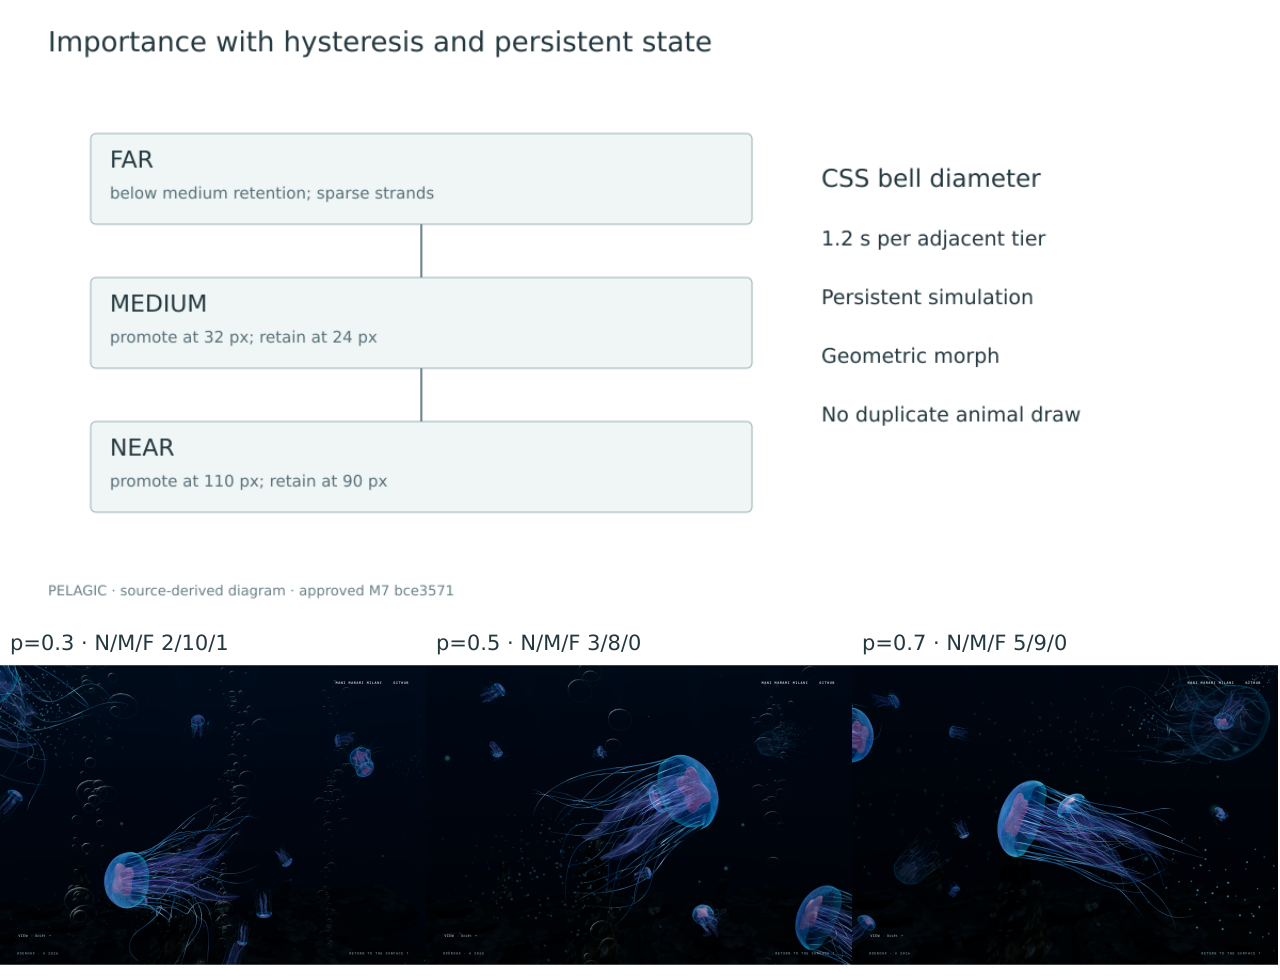
\includegraphics[keepaspectratio,alt={Figure 6. Projected-size detail thresholds and actual population snapshots under identical viewport/DPR settings. N/M/F are near/medium/far counts. Different journey positions are not a forced same-pose tier ablation. CSS thresholds do not change with DPR.}]{figures/F06-lod.png}}
\caption{Figure 6. Projected-size detail thresholds and actual
population snapshots under identical viewport/DPR settings. N/M/F are
near/medium/far counts. Different journey positions are not a forced
same-pose tier ablation. CSS thresholds do not change with DPR.}
\end{figure}

\textbf{Algorithm 3 --- importance detail.}

\begin{Shaded}
\begin{Highlighting}[]
\NormalTok{read existing main and distant route poses}
\NormalTok{test conservative animal bounds against camera frustum}
\NormalTok{compute CSS bell diameter; choose hysteretic target tier}
\NormalTok{advance continuous detail without pause debt}
\NormalTok{reuse persistent spines; sample adjacent prepared surface levels}
\NormalTok{morph geometry and strand widths, not two full animal renderings}
\NormalTok{assign finite light/fleck resources by visible importance}
\NormalTok{retain normal activation eligibility and approved near presentation}
\end{Highlighting}
\end{Shaded}

\section{13. Camera journey and
exploration}\label{camera-journey-and-exploration}

The camera is input-driven. Wheel line/page units normalize to CSS-pixel
intent; touch and keyboard inputs reach the same bounded follower.
Opposite intent cancels queued travel without teleporting the camera. No
production autoplay advances the journey when the visitor stops.

With progress error \(e=s_{target}-s\), gain \(g\), speed bound
\(v_m=0.14\), acceleration bound \(a_m=1.4\) and \(h=1/240\), equation
(13), \textbf{CODE-EQUIVALENT}, is

\[
\begin{aligned}
v_d&=\operatorname{sgn}(e)\min[v_m\tanh(g|e|),\sqrt{2a_m|e|}],\\
v^+&=v+\operatorname{clamp}(v_d-v,-a_mh,a_mh),\\
s^+&=s+hv^+.
\end{aligned}
\]

The target stays at most 0.075 ahead/behind progress and within
\([0,1]\). Balanced gain is 72; cinematic/responsive use 52/92. Tiny
residual motion snaps to exact rest only within the allowed braking
step. A legacy \texttt{ProgressSpring} class remains in source but does
not define current production travel.

Each view bakes 1,201 poses. For a scalar coordinate over one authored
segment, let \(p\) be the starting value, \(\Delta\) its difference, and
\(m,n\) the endpoint tangents multiplied by segment span. Equation (14),
\textbf{CODE-EQUIVALENT}, is

\[
P(t)=p+mt+(10\Delta-6m-4n)t^3
 +(-15\Delta+8m+7n)t^4+(6\Delta-3m-3n)t^5.
\]

Interior tangents use a monotone harmonic construction; endpoint
tangents are zero. Authoring angles unwrap before conversion to
hemisphere-continuous quaternions. Runtime sampling linearly
interpolates position and spherically interpolates quaternion. Thus the
authoring polynomial is smooth, while the finite sampled playback is an
approximation to it---not an analytic continuous quaternion spline.

Documentary, Drift, Intimate and Deep expose different authored tracks.
Explore temporarily gives the visitor observer control without
rebuilding the ocean. Idle holds the observer and journey while animals
continue moving. S6 shows view changes and Explore; the paper does not
reinterpret those controls as simulation steering or a new camera
design.

\section{14. Shared optical compositor}\label{shared-optical-compositor}

One ocean image supplies all active optical effects.
\texttt{LiveOceanLens} owns a full drawing-buffer RGBA16F target, a
depth attachment, and the output material. The scene is rendered into
that target without the lens in its input. Thermal shimmer and bubble
slots sample that clean source; idle may then replace local output with
its own clean-source lookup. There is no recursive color feedback.

This ordering has a cost and a limitation. The output adds a
screen-sized pass when optical content is active; idle also advances its
small persistent field. However, overlapping optical effects do not
solve nested ray transport. Each effect sees the same unmodified ocean
source. The blend can preserve an attractive image without representing
light that physically traversed every intervening surface.

The target uses renderer sample count and linear color. Tone/output
state is restored around preparation and rendering, including failure
paths. A tiny scratch target is used during idle preparation and then
disposed. Ready state is published after a valid first optical draw, not
merely after allocating a material. Figure 7 diagrams source versus
output ownership.

\begin{figure}
\centering
\pandocbounded{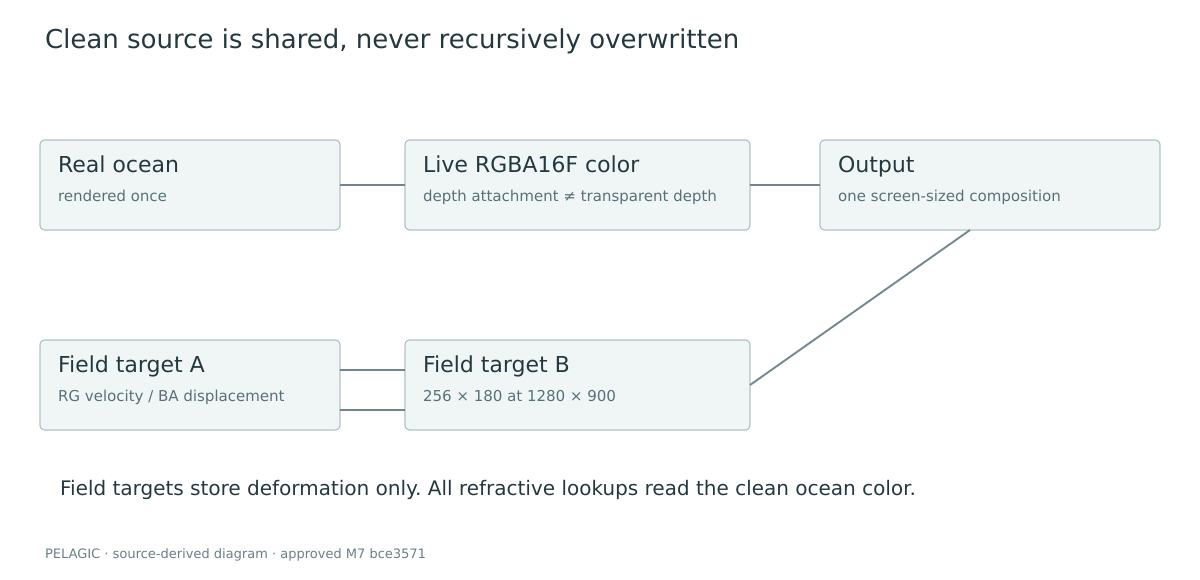
\includegraphics[keepaspectratio,alt={Figure 7. Shared clean-image compositor. The output is never sampled as its own input; idle field ping-pong stores state, not ocean color.}]{figures/F07-compositor.png}}
\caption{Figure 7. Shared clean-image compositor. The output is never
sampled as its own input; idle field ping-pong stores state, not ocean
color.}
\end{figure}

\textbf{Algorithm 4 --- optical frame.}

\begin{Shaded}
\begin{Highlighting}[]
\NormalTok{advance bounded idle field, if needed}
\NormalTok{prepare active thermal/bubble domains}
\NormalTok{if no optical domain and no visible idle: render ocean directly}
\NormalTok{otherwise:}
\NormalTok{    resize clean target to actual drawing buffer}
\NormalTok{    render the real ocean once into clean target}
\NormalTok{    sample clean image for thermal and bounded bubble slots}
\NormalTok{    if idle visible: evaluate liquid field and clean{-}image displacement}
\NormalTok{    render output once; restore renderer state even after errors}
\end{Highlighting}
\end{Shaded}

\section{15. Bubble optics and
lifetime}\label{bubble-optics-and-lifetime}

For lens-local origin \(o\), direction \(d\) and ellipsoid radii vector
\(r\), define \(O=o/r\), \(D=d/r\). Equation (15),
\textbf{CODE-EQUIVALENT}, is

\[
\begin{aligned}
A&=D\cdot D,\quad B=O\cdot D,\quad C=O\cdot O-1,\\
t_e&=\frac{-B-\sqrt{\max(B^2-AC,10^{-6})}}{A},\\
n&=\operatorname{normalize}[(o+t_ed)/r^2].
\end{aligned}
\]

The shader transforms the normal by the appropriate normal matrix and
refracts in metric view space. A second analytic intersection finds the
exit; a second refraction computes the outgoing direction. This is
different from deforming only a visible lens mesh while leaving the
source image unchanged.

Equation (16), \textbf{CODE-EQUIVALENT} for the projection core, uses
exit point \(E_v\), outgoing view ray \(D_o\), scene view-depth \(z_s\),
and camera projection \(P\):

\[
\begin{aligned}
z_i&=\max(z_s,E_{v,z}-6),\\
\ell&=\max\left(0,\frac{z_i-E_{v,z}}{\min(D_{o,z},-0.05)}\right),\\
q&=P(E_v+\ell D_o,1),\\
uv_r&=(q_x/(2q_w)+1/2,\;1/2-q_y/(2q_w)).
\end{aligned}
\]

The actual code guards the homogeneous denominator, grazing rays, source
borders and depth tests. Bubble lookup displacement is capped to
\(\sqrt{2}\,0.008\) in UV length before further masks. The virtual image
plane six units behind the exit is explicitly approximate, especially
for transparent animals that do not write depth. A depth texture is not
translucent depth, and its attachment is not proof that the selected
backend resolves it correctly. The pinned WebGL multisample limitation
is recorded in the supplement.

Five refractive heroes accompany 384 cheap ambient films. Seeded
lifetimes, stream packets, aspect-changing shape and modest drift make a
bounded passage, not a permanent screen of lenses. Only heroes perform
the analytic optical lookup. Authored index ratios are softened rather
than using a literal water/air ratio that would require unavailable
reflected scene rays at grazing angles. Figure 8 and S5 expose the image
bending and its limitations in motion.

\begin{figure}
\centering
\pandocbounded{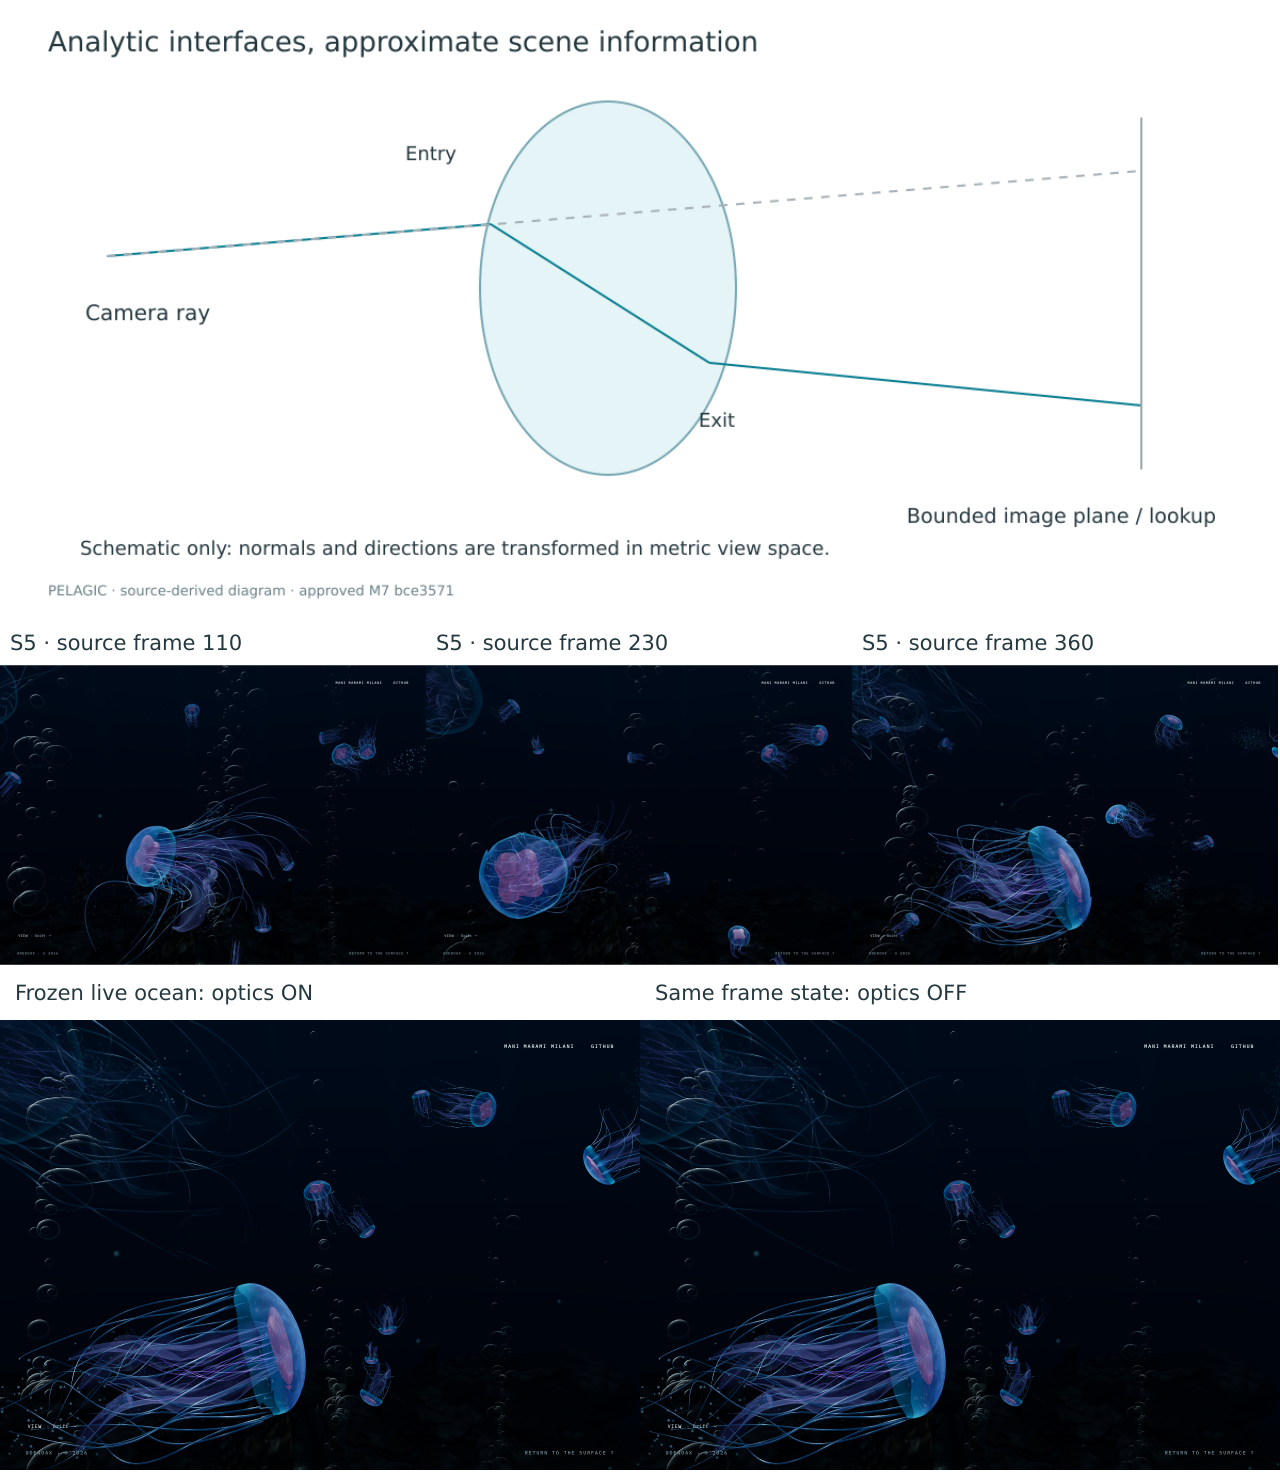
\includegraphics[keepaspectratio,alt={Figure 8. Analytic-interface schematic, three actual S5 browser frames and a frozen optics-on/off diagnostic. The virtual image plane is approximate; disabling hero refraction through the existing review API retains ambient bubble films. These are live-color distortions, not scene reconstruction.}]{figures/F08-refraction.png}}
\caption{Figure 8. Analytic-interface schematic, three actual S5 browser
frames and a frozen optics-on/off diagnostic. The virtual image plane is
approximate; disabling hero refraction through the existing review API
retains ambient bubble films. These are live-color distortions, not
scene reconstruction.}
\end{figure}

\section{16. Abyssal sanctuary and participating-media
approximation}\label{abyssal-sanctuary-and-participating-media-approximation}

The deep scene uses a dark basalt basin, connected shelves, a recessed
channel, one principal sulfide structure, secondary spires and sparse
vent-associated life. These are procedural and instanced artistic forms,
not a surveyed site. Processed Rock 07 scan luminance
(\citeproc{ref-polyhaven}{Poly Haven, n.d.}) contributes mineral
variation. The active geology material is \texttt{MeshBasicNodeMaterial}
with an authored surface-gradient lighting response; calling it a
calibrated PBR BRDF would be incorrect. Scanned detail and physically
motivated placement do not change that.

The plume maintains fixed-capacity position, velocity, age, lifetime and
size arrays. It is pre-established at construction rather than emitted
as a first- visit burst. Nearby mineral packets share spatially related
eddies. In equation (17), \textbf{CODE-EQUIVALENT} for selected updates,
sampled current \(U\) is filtered into \(U_f\), then a target plume
velocity \(V_d\) is followed:

\[
\begin{aligned}
U_f^+&=U_f+[\operatorname{clamp}(U,-0.65,0.65)-U_f](1-e^{-h/0.85}),\\
V^+&=V+(V_d-V)(1-e^{-kh}),\quad X^+=X+hV^+.
\end{aligned}
\]

\(k=2.1\) for smoke and 1.2 otherwise. Smoke's vertical target includes
\(1.6e^{-0.18a}+0.045\) plus filtered vertical current. Lateral
entrainment grows with height. These are \textbf{ART-DIRECTION
HEURISTICS} when interpreted as plume physics: no temperature, pressure
or buoyancy conservation is solved.

Localized thermal domains reuse the optical output. Their world-space
pattern and bounded projection produce shimmer without a second scene
render. A single pooled animal-derived lighting contribution changes
owner through zero rather than sliding an unrelated bright point across
the floor. Channel-dependent distance attenuation blends toward
directional water radiance. This is not volumetric multiple scattering
or measured ocean image formation.

\begin{figure}
\centering
\pandocbounded{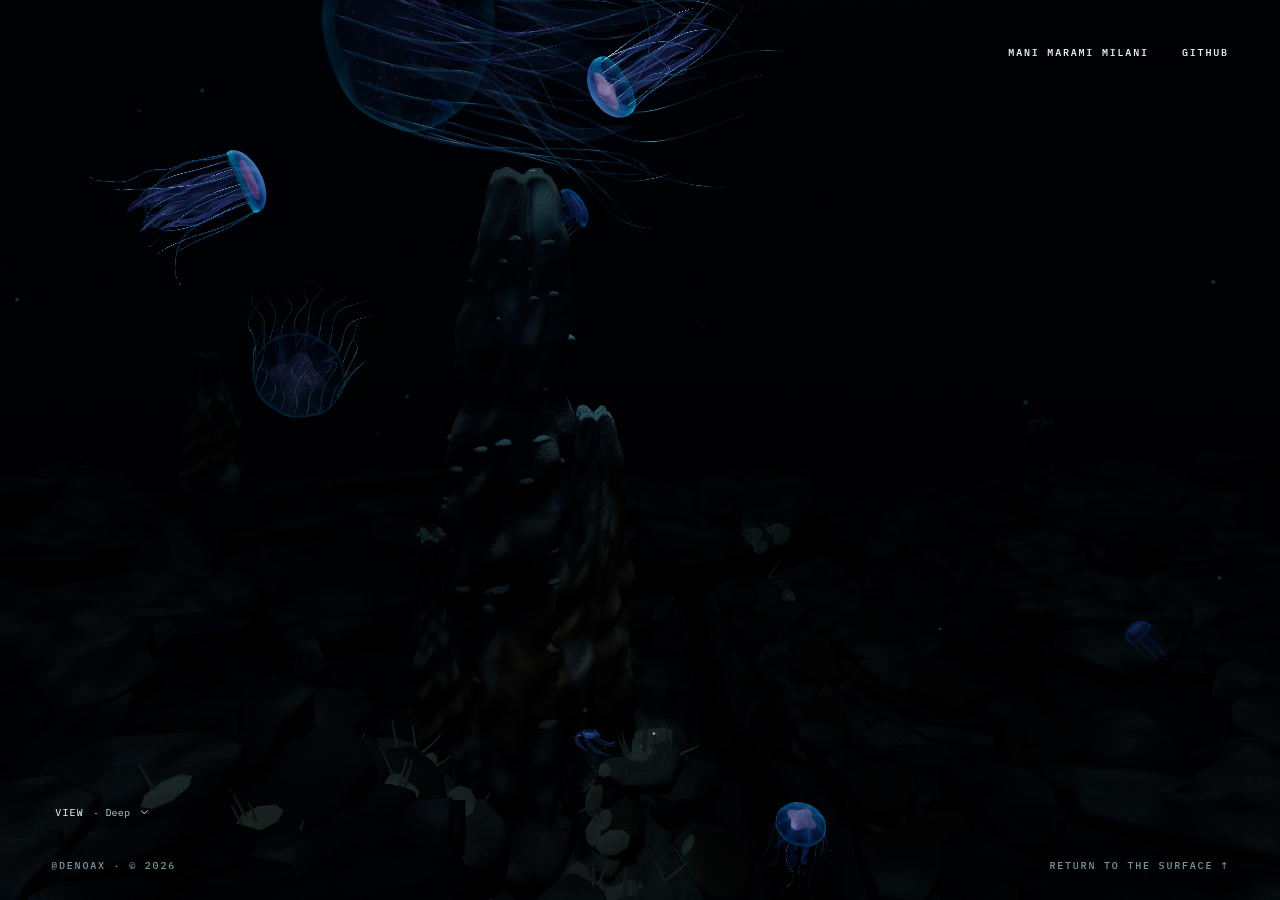
\includegraphics[keepaspectratio,alt={Figure 9. Approved sanctuary at the publication runtime: procedural geology, localized plume and restrained life.}]{figures/F09-sanctuary.jpg}}
\caption{Figure 9. Approved sanctuary at the publication runtime:
procedural geology, localized plume and restrained life.}
\end{figure}

\section{17. Idle state and implicit liquid
topology}\label{idle-state-and-implicit-liquid-topology}

Idle is a mode of the shared compositor, not another WebGL canvas. The
semantic \texttt{IdleScreen} contains no renderer. A 30-second
inactivity policy requests entry; readiness and reduced-motion
conditions govern whether it appears. Pointer motion deforms the active
film without dismissing it. Click/tap or the defined keyboard actions
initiate dismissal and consume the event before it becomes an animal
click. The ocean continues beneath a held camera pose.

The clock uses two independent canvas textures. Clone-sharing a texture
source would not supply independent old/new masks in this Three.js
version. Digits occupy fixed cells while retaining the font's
proportional shapes. Landscape uses HH:MM; portrait stacks hours and
minutes. Eight contact sites are found from the project's own
low-resolution clock mask, not from ocean readback.

Equation (18) is a \textbf{CONTINUOUS ABSTRACTION} of the scalar
topology:

\[
F(u)=a\,S_{0.12,0.95}\left(
G(u-\Delta)+\sum_j D_j(u-\Delta)+\sum_j N_j(u-\Delta)+\sum_j R_j(u-\Delta)
\right).
\]

\(a\) is entry/exit amount; \(G\) is the mapped, locally grown/eroded
glyph; \(D_j,N_j,R_j\) are droplet, neck and reservoir/bulge
contributions. The actual function includes conditionals for changed
cells, colon growth, front arrival, old/new stroke mapping and exit. It
is not accurately represented by simply crossfading two text images.
Gaussian-like additive masses create connected boundaries, but their sum
is not a material-volume conservation law.

The field is evaluated at the sample and four offsets. In equation (19),
\textbf{CODE-EQUIVALENT}, \(e=(1.7/W,1.7/H)\) and

\[
\begin{aligned}
g&=(F(u+(e_x,0))-F(u-(e_x,0)),\;
F(u+(0,e_y))-F(u-(0,e_y))),\\
n&=\operatorname{normalize}(-16g_x,-16g_y,1),\\
\delta u&=0.035\,n_{xy}(H/W,1)F(u)\,S(a)\,S_{0,0.06}(border).
\end{aligned}
\]

The difference is intentionally not divided by \(2e\). Its scale and the
factor 16 form an artistic normal construction. The resulting lookup
samples the current clean ocean color at clamped \(u+\delta u\). Small
normal-driven light and luminance adaptation support the material; they
do not substitute for live image displacement. S8--S12 show formation,
contact, interaction, minute change and dismissal at normal presentation
size.

\begin{figure}
\centering
\pandocbounded{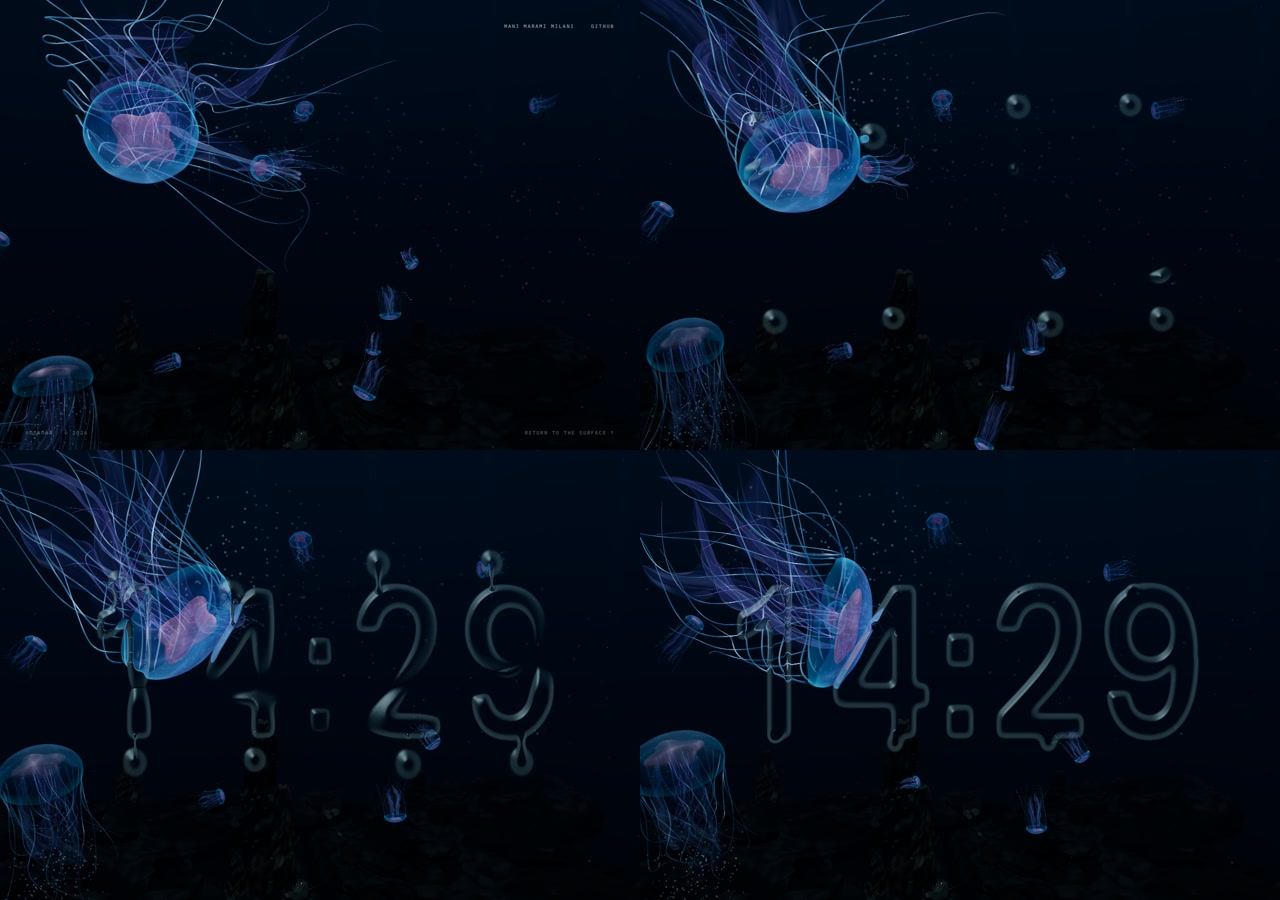
\includegraphics[keepaspectratio,alt={Figure 10. Normal-size clock contact and merge sequence. The supplement records actual timing and warns against interpreting the authored neck as conserved fluid.}]{figures/F10-contact.jpg}}
\caption{Figure 10. Normal-size clock contact and merge sequence. The
supplement records actual timing and warns against interpreting the
authored neck as conserved fluid.}
\end{figure}

\section{18. Persistent deformation and event
choreography}\label{persistent-deformation-and-event-choreography}

The paired field stores velocity in RG and displacement in BA, signed
around zero in RGBA16F. Its long dimension is 256, with a minimum of 64
samples on either axis. It is small state, not a downsampled fake ocean.
Current ocean color stays in the separate full-resolution optical
target.

For screen coordinate \(u\), first read previous velocity \(V_0\),
backtrace \(p=u-0.42hV_0\), and sample state \((V,D)\) plus its
four-neighbor average \((\bar V,\bar D)\). Equation (20),
\textbf{CODE-EQUIVALENT}, gives the core step:

\[
\begin{aligned}
V'&=\operatorname{clamp}_{[-0.58,0.58]}
\{[0.88V+0.12\bar V+h(36(\bar D-D)-5.5D)]e^{-2.8h}
+3.2h\,V_pBI\},\\
D'&=\operatorname{clamp}_{[-0.17,0.17]}(D+hV').
\end{aligned}
\]

\(V_p\) is bounded pointer velocity, \(B\) a Gaussian segment brush,
\(I\) fresh-input presence. A queued bounded event impulse is added to
\(V'\) after its clamp and before displacement integration; an edge
envelope multiplies the final state. That order is material: the first
clamp alone is not an absolute bound after the event term. The method is
a spring/advection construction, not incompressible Navier--Stokes, and
no pressure projection is performed.

Entry contact follows the facing mask surface, not an interior stroke
anchor. The existing M7.2 choreography gives the approaching surfaces a
visible gap, creates a narrow connection, then transfers and settles.
Let \(b=S(age/0.65)\) and \(T=S((t-0.29)/0.58)\) after the per-site
contact time. Equation (21), \textbf{CODE-EQUIVALENT} for entry radius,
is

\[
r=(0.034+0.003(i\bmod3))\sqrt{(1-T)b}.
\]

The source's scalar \texttt{mass=1-T} is a choreography bookkeeping
quantity, not a physical integral of the implicit field. Stroke growth
also draws from an explicit authored reservoir. Dismissal creates a
throat that narrows, breaks and recoils before the remaining field
disappears. Events trigger modest field impulses once per site and reset
on mode changes. Figure 11 shows exit at normal size; enlarged
diagnostics alone would overstate its readability.

\begin{figure}
\centering
\pandocbounded{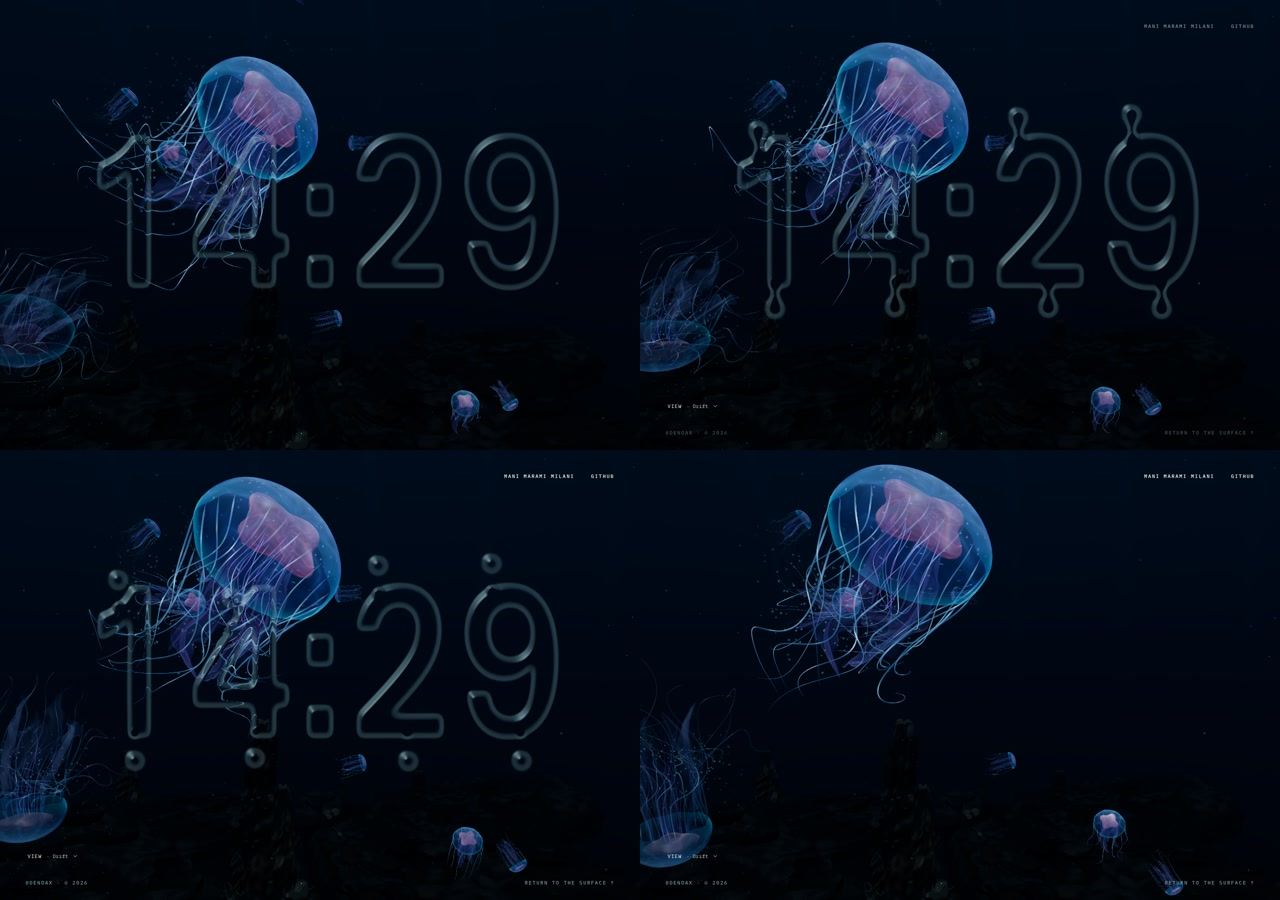
\includegraphics[keepaspectratio,alt={Figure 11. Throat narrowing, separation and recovery during approved M7.2 dismissal. Actual browser frames, not generated liquid artwork.}]{figures/F11-pinch.jpg}}
\caption{Figure 11. Throat narrowing, separation and recovery during
approved M7.2 dismissal. Actual browser frames, not generated liquid
artwork.}
\end{figure}

\textbf{Algorithm 5 --- liquid frame.}

\begin{Shaded}
\begin{Highlighting}[]
\NormalTok{read idle intent; reset only choreography/input bookkeeping on state change}
\NormalTok{refresh masks only for layout or minute changes}
\NormalTok{advance bounded controller time and compute local contact/drop/neck state}
\NormalTok{enqueue each contact or break impulse once}
\NormalTok{advance persistent field through ping{-}pong targets}
\NormalTok{evaluate mapped glyph + implicit masses at displaced coordinates}
\NormalTok{derive artistic thickness normal; sample current clean ocean image}
\NormalTok{blend optical presentation without feeding output color back into state}
\end{Highlighting}
\end{Shaded}

\section{19. Lifecycle and timing}\label{lifecycle-and-timing}

Subsystems deliberately reject or cap suspension debt. The idle
controller clears its accumulator when hidden. Its per-call duration is
at most 0.05 s; the tissue path also has finite-duration guards. These
are stability policies, not exact real-time continuation through a
background pause.

Equation (22), \textbf{CODE-EQUIVALENT} for the idle accumulator with
\(h=1/60\), is

\[
A'=\min(A+\min(dt,0.05),3h),\quad
N=\min(3,\lfloor(A'+10^{-10})/h\rfloor),\quad A^+=A'-Nh.
\]

Hidden/invalid-input branches clear debt before this expression. The
renderer is serialized to avoid concurrent frame work. Idle shader
linking may continue while ordinary frames render, but the optical
output is not exposed until its first valid draw. Resize changes target
dimensions and invalidates field state as required; teardown waits for
in-flight ownership before disposing resources.

\textbf{Algorithm 6 --- bounded lifecycle.}

\begin{Shaded}
\begin{Highlighting}[]
\NormalTok{if hidden or invalid input: clear relevant debt/input latch; do not catch up}
\NormalTok{otherwise cap admitted duration and accumulate at most the allowed steps}
\NormalTok{run fixed steps, retaining only a fractional remainder}
\NormalTok{serialize scene/output work and restore renderer state on exceptions}
\NormalTok{publish readiness only after successful preparation}
\NormalTok{on teardown: stop listeners, settle in{-}flight ownership, dispose once}
\end{Highlighting}
\end{Shaded}

\section{20. Implementation and artifact
boundary}\label{implementation-and-artifact-boundary}

The locked software stack is React 19.2.0, Three.js 0.175.0 and Vite
6.4.2. The build uses the existing static client/Sites packaging path;
publication does not modify its worker or deployment configuration.
Scientific diagrams, plots, metadata and portable browser tools are
publication additions only. The source manifest checks byte parity of
runtime files against the approved commit rather than inferring parity
from a successful build.

The repository contains historical modules and assets that are no longer
active. Import paths decide implementation truth. In particular, the old
idle renderer and old camera cannot be cited as current simply because
their files remain. The provenance audit separates active scanned
albedo, archived models, generated graphics-recovery artwork, original
publication captures and external reference-only material.

\section{21. Experimental methodology}\label{experimental-methodology}

Fresh performance measurements run separately from screenshots, video
capture, encoding, builds and tests. The recorded quantity is the
interval between completed asynchronous ocean-frame callbacks. It is not
a GPU timestamp or a measurement of shader duration. The harness records
its matching method and rejects empty samples. Browser scheduling,
compositor cadence, CPU work and driver submission all contribute.

The minimum scenario set is opening, midwater, bubble passage,
sanctuary, Explore, settled idle and active idle manipulation. Each
record includes runtime SHA, browser and backend, hardware, viewport,
drawing buffer, DPR, quality/bloom state, warm-up, duration and raw
intervals. A deterministic random seed makes initial conditions more
comparable; real-time interactive trajectories still depend on
scheduling. Existing development hooks select review states; they do not
authorize changed runtime algorithms.

The fresh-results table is generated from retained data, not copied from
a milestone report. Median, p95, maximum and counts above 50 ms are
reported together. Adverse intervals remain in the data. A quiet
repeated frame does not prove that an active transition is equally
cheap. Conversely, a capture-induced stall is not silently used as
evidence of ordinary runtime cost.

\section{22. Results}\label{results}

\subsection{22.1 Correctness and
invariants}\label{correctness-and-invariants}

A clean dependency installation succeeded. The first pre-build suite
passed 129 of 130 tests; the remaining test required generated packaging
output. Building first satisfied that prerequisite, after which all 130
existing tests passed. The approved-motion check covered 720 frames and
24 exact checkpoints; the legacy default-animal parity check covered 240
frames and eight checkpoints. These narrow checks establish their stated
comparisons, not biological correctness or universal visual acceptance.

\subsection{22.2 Visual evidence}\label{visual-evidence}

The figure set and S1--S12 motion gallery expose separate claims:
anatomy and pulse, turn-related lag, current activation, detail
transitions, bubble optics, camera modes, sanctuary behavior, and the
idle lifecycle. Actual browser frames are distinguished from
source-derived diagrams. Normal-size merge and pinch footage is included
because a zoomed crop can make an otherwise invisible event appear
convincing. Human art-direction approval remains distinct from automated
correctness and from any unperformed perception study.

\subsection{22.3 Fresh performance}\label{fresh-performance}

Table 3 and Figure 12 are generated from the fresh benchmark record.
They use the exact approved runtime and preserve all raw adverse
samples. Measurements are frame intervals, not GPU timings. No
comparative performance claim against other projects is made.

\textbf{Table 3. Fresh approved-runtime frame intervals (milliseconds).}

{\def\LTcaptype{none} % do not increment counter
\begin{longtable}[]{@{}lrrrrr@{}}
\toprule\noalign{}
Scenario & Median & p95 & Maximum & \textgreater50 ms & Frames \\
\midrule\noalign{}
\endhead
\bottomrule\noalign{}
\endlastfoot
opening & 16.70 & 18.60 & 28.80 & 0 & 1800 \\
midwater & 16.70 & 17.80 & 27.20 & 0 & 1800 \\
bubble passage & 16.70 & 18.70 & 65.30 & 1 & 1798 \\
sanctuary & 16.70 & 18.00 & 25.90 & 0 & 1800 \\
Explore & 16.70 & 18.50 & 31.80 & 0 & 1800 \\
settled M7 & 16.70 & 17.90 & 26.00 & 0 & 1800 \\
M7 manipulation & 16.70 & 18.20 & 30.00 & 0 & 1803 \\
\end{longtable}
}

Actual NVIDIA WebGL2; 1280×900 viewport and drawing buffer; DPR 1; bloom
off. Eleven-second initial warm-up plus scene/idle warm-up; 30-second
measurement per case. Existing development hooks select the approved
runtime states. These are render-completion intervals, not GPU timings.
Single-run observations, not confidence intervals. Bubble passage
includes its natural decay. No capture or video encoding during timing.

The measured browser is Brave/Chromium 152.0.7977.76, with ANGLE OpenGL
ES 3.2 on an NVIDIA RTX 4070. The Linux host uses an Intel Core
i5-14600K and 62.5 GiB RAM. Its local llama service remained running
consistently; this run does not isolate service contention. Existing
development fixtures hold DPR at 1 without adaptive downshift. Median
and p95 use sorted samples at floor(0.5n) and floor(0.95n),
respectively. The bubble case retained one 65.3 ms interval; its cause
is not established. The natural bubble window may end within the
30-second observation. Draw-call snapshots were not sampled in that
timing run; separate diagnostic population records must not be relabeled
as simultaneous benchmark draw counts. Raw arrays and environment
records are retained in \texttt{results/benchmark.json}.

\begin{figure}
\centering
\pandocbounded{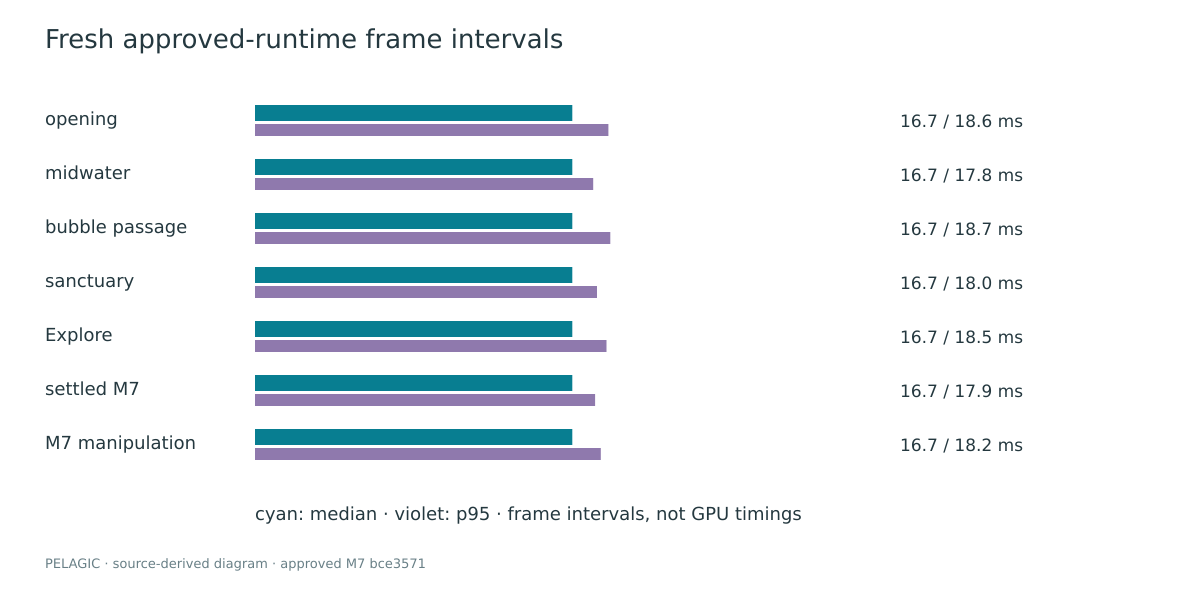
\includegraphics[keepaspectratio,alt={Figure 12. Fresh publication-runtime median and p95 frame intervals. Labels identify scene and measurement conditions; no screenshot/video work runs during timing.}]{figures/F12-performance.png}}
\caption{Figure 12. Fresh publication-runtime median and p95 frame
intervals. Labels identify scene and measurement conditions; no
screenshot/video work runs during timing.}
\end{figure}

\subsection{22.4 Compatibility scope}\label{compatibility-scope}

\textbf{Table 4. Compatibility scope of this publication, not a general
support promise.}

{\def\LTcaptype{none} % do not increment counter
\begin{longtable}[]{@{}
  >{\raggedright\arraybackslash}p{(\linewidth - 2\tabcolsep) * \real{0.5000}}
  >{\raggedright\arraybackslash}p{(\linewidth - 2\tabcolsep) * \real{0.5000}}@{}}
\toprule\noalign{}
\begin{minipage}[b]{\linewidth}\raggedright
Environment
\end{minipage} & \begin{minipage}[b]{\linewidth}\raggedright
Scope
\end{minipage} \\
\midrule\noalign{}
\endhead
\bottomrule\noalign{}
\endlastfoot
NVIDIA RTX 4070, Brave/Chromium, WebGL2 & actual graphics path used for
primary captures and fresh results \\
Narrow and 390×844 portrait viewports & browser emulation; not
physical-mobile validation \\
Hardware WebGPU full ocean & NOT TESTED in this publication; legacy
full-ocean issue remains separate \\
SwiftShader/software WebGPU & NOT TESTED in this publication unless an
explicitly separate record is supplied \\
Safari, Firefox, iOS/Android hardware & NOT TESTED \\
\end{longtable}
}

\section{23. Ablations and rejected
approaches}\label{ablations-and-rejected-approaches}

The supplement distinguishes controlled same-runtime ablations from
historical changes. Turning a current feature off isolates a
contribution but does not necessarily provide a viable alternative
implementation. A historical before/after may change several systems and
cannot support a causal speedup claim without controlling those
differences.

\textbf{Table 5. Engineering questions and evidence interpretation.}

{\def\LTcaptype{none} % do not increment counter
\begin{longtable}[]{@{}
  >{\raggedright\arraybackslash}p{(\linewidth - 4\tabcolsep) * \real{0.3333}}
  >{\raggedright\arraybackslash}p{(\linewidth - 4\tabcolsep) * \real{0.3333}}
  >{\raggedright\arraybackslash}p{(\linewidth - 4\tabcolsep) * \real{0.3333}}@{}}
\toprule\noalign{}
\begin{minipage}[b]{\linewidth}\raggedright
Comparison
\end{minipage} & \begin{minipage}[b]{\linewidth}\raggedright
What it can establish
\end{minipage} & \begin{minipage}[b]{\linewidth}\raggedright
What it cannot establish
\end{minipage} \\
\midrule\noalign{}
\endhead
\bottomrule\noalign{}
\endlastfoot
Optical compositor enabled/disabled at matched state & live image
displacement and added presentation & physically correct multilayer
refraction \\
Connected particulate visible/hidden & local visual contribution &
hydrodynamic accuracy or perceptual preference \\
Persistent field at rest/after pointer/recovery & remembered deformation
and settling & conserved liquid volume \\
Historical independent camera corrections vs bounded pose path & why
ownership was simplified & an isolated benchmark speedup \\
Historical separate idle renderer vs shared M7 & architectural change
and source ownership & universal browser compatibility \\
\end{longtable}
}

Rejected giant dark lenses, bright repetitive geology and early camera
corrections are presented as development history, not as straw-man
competitors. The later Asset2 experiment missed requested image-metric
improvements and its optional GTAO path encountered unhelpful depth
sampling. It is not promoted to approved runtime or used as proof that
ambient occlusion improved the artwork. The input-boundary defect behind
an earlier idle failure is also distinguished from a shader diagnosis:
malformed synthetic pointer data could poison state, so validation had
to identify the first invalid input rather than sanitize final geometry.

\section{24. Limitations}\label{limitations}

Pelagic is not calibrated to a species, a measured ocean volume, or
physical tissue properties. Its bell and folds are procedural art
direction. Constraint iterations and clearance heuristics can reduce,
but not eliminate, intersections. The appendages do not solve continuum
elasticity or complete self-collision. Route separation is not a
validated collective-behavior model.

Current, wake and plume fields are bounded approximations. Their shared
timing and spatial dependence improve coherence, but there is no
fluid--structure coupling, pressure solve, mass conservation, thermal
transport or prediction of real vent behavior. Distance-dependent water
appearance is not a validated participating-media reconstruction.
Geological textures contribute surface detail without converting
authored lighting into a measured BRDF.

Image-space optics have finite information. They cannot recover
offscreen or occluded radiance. Transparent tissue lacks its own
resolved depth layer. Virtual planes, displacement caps, grazing fades
and softened indices are deliberate compromises. Multiple optical
effects share a clean source rather than recursively transporting light.
The pinned WebGL depth-resolution issue further limits occlusion
confidence; attachment presence must not be advertised as correct depth
behavior.

The liquid clock is a two-dimensional scalar presentation with authored
contact timing and small persistent deformation. Its necks and
reservoirs do not prove conserved volume. Resize may reset local field
state. Hidden-tab time is discarded, not physically simulated.
Preparation can still impose one-time driver work; steady-state frame
intervals do not erase that cost.

The hardware matrix is narrow. Results on one NVIDIA desktop and
emulated viewports do not establish mobile performance, Safari
compatibility, or a fixed frame budget on all machines. Visual approval
is Mani's artistic judgment, not a controlled user study. No peer-review
or priority claim accompanies this independent technical preprint.

\section{25. Reproducibility}\label{reproducibility}

Use the recorded runtime commit, not an unspecified current main branch.
Install the lockfile, build, run tests and parity checks, then start the
local review server. \texttt{REPRODUCIBILITY.md} gives portable commands
and tool versions. The publication browser harness records scenario
state and metadata separately from video. Its benchmark mode never
captures frames. Large source clips and raw capture material remain
outside normal Git; curated figures, lightweight GIFs and numerical
records fit the publication media budget.

The release staging directory contains the paper and supplement PDFs, a
reproducibility archive, supplemental motion archive, prepared arXiv
source and SHA-256 manifest. These are local deliverables, not evidence
of an issued GitHub release, DOI or arXiv submission. The currently
public ocean is linked for visitors with an explicit version caveat.
Publication requires a separate author approval step.

\section{26. AI assistance and
provenance}\label{ai-assistance-and-provenance}

Mani Marami Milani directed and reviewed the artwork. Codex/OpenAI
models assisted with implementation, source auditing, documentation,
test tooling and publication preparation. This disclosure is not an
independent verification of every generated statement; the source map,
measured data and human review gate remain necessary. Existing generated
artwork is used for graphics recovery or reduced-motion fallback, not
substituted for successful runtime motion evidence.

Original code is MIT licensed; original publication text, diagrams and
project-generated screenshots/media are CC BY 4.0. Third-party code,
fonts, textures and archived models retain their own terms. This policy
does not relicense external research material. Scientific figures from
other authors are linked or cited, not copied into the publication's
original figure set.

\section{27. Conclusion}\label{conclusion}

Pelagic's useful result is an inspectable connection between an
organism, its surrounding water and an optical interface. Shared state,
bounded time, consistent coordinate spaces and explicit resource
ownership matter as much as individual shading techniques. The approved
system preserves a procedural animal through motion and detail changes,
lets its environment respond, and uses the real moving ocean as the
source for liquid optics.

The artifact makes those decisions reproducible without overstating
them. Its strongest claims are source-level integration, demonstrated
behavior and measured performance under stated conditions. Its physical
and compatibility limits remain visible. Further biological calibration,
more complete optical transport and broader hardware validation would be
separate work, not implied achievements of this publication.

\section{References}\label{references}

\protect\phantomsection\label{refs}
\begin{CSLReferences}{1}{1}
\bibitem[\citeproctext]{ref-blinn1982}
Blinn, James F. 1982. {``A Generalization of Algebraic Surface
Drawing.''} \emph{ACM Transactions on Graphics} 1 (3): 235--56.
\url{https://doi.org/10.1145/357306.357310}.

\bibitem[\citeproctext]{ref-fluidglass}
{chiuhans111}. n.d. \emph{FluidGlass}.
\url{https://github.com/chiuhans111/fluidglass}.

\bibitem[\citeproctext]{ref-costello2021}
Costello, John H., Sean P. Colin, John O. Dabiri, Brad J. Gemmell,
Kelsey N. Lucas, and Kelly R. Sutherland. 2021. {``The Hydrodynamics of
Jellyfish Swimming.''} \emph{Annual Review of Marine Science} 13:
375--96. \url{https://doi.org/10.1146/annurev-marine-031120-091442}.

\bibitem[\citeproctext]{ref-gemmell2013}
Gemmell, Brad J., John H. Costello, Sean P. Colin, et al. 2013.
{``Passive Energy Recapture in Jellyfish Contributes to Propulsive
Advantage over Other Metazoans.''} \emph{Proceedings of the National
Academy of Sciences} 110 (44): 17904--9.
\url{https://doi.org/10.1073/pnas.1306983110}.

\bibitem[\citeproctext]{ref-muller2007}
Müller, Matthias, Bruno Heidelberger, Marcus Hennix, and John Ratcliff.
2007. {``Position Based Dynamics.''} \emph{Journal of Visual
Communication and Image Representation} 18 (2): 109--18.
\url{https://doi.org/10.1016/j.jvcir.2007.01.005}.

\bibitem[\citeproctext]{ref-aurelia}
Niehus, Niklas. n.d. \emph{Aurelia}.
\url{https://github.com/holtsetio/aurelia}.

\bibitem[\citeproctext]{ref-polyhaven}
Poly Haven. n.d. \emph{Rock 07}. \url{https://polyhaven.com/a/rock_07}.

\bibitem[\citeproctext]{ref-three175}
Three.js contributors. 2025. \emph{{Three.js r175} Source and Rendering
Implementation}. \url{https://github.com/mrdoob/three.js/tree/r175}.

\bibitem[\citeproctext]{ref-wyman2005}
Wyman, Chris. 2005. {``An Approximate Image-Space Approach for
Interactive Refraction.''} \emph{ACM Transactions on Graphics} 24 (3):
1050--53. \url{https://doi.org/10.1145/1073204.1073310}.

\end{CSLReferences}

\section{Appendix A. Reading the
artifact}\label{appendix-a.-reading-the-artifact}

\texttt{source-map.md} connects every equation to the fixed runtime.
\texttt{notation.md} defines symbols and spaces. The claim ledger
separates source proof, benchmark proof, observation and heuristics. The
supplement contains motion descriptions, extended measurements,
ablations and historical negative results. The manifest records file
hashes and distinguishes runtime SHA from publication SHA.

Figures 1, 9--11 are runtime evidence; Figures 2--8 include original
explanatory diagrams or source-derived plots. Figures 4, 6 and 8 also
include labeled browser frames, as their captions state. Figure 12 is
generated from fresh raw measurements. No diagram is represented as a
rendered result.

\end{document}
